\documentclass[10pt]{article}
\usepackage{hyperref}
% \renewcommand{\familydefault}{\sfdefault}
% \usepackage[utf8]{inputenc}
\usepackage{graphicx}
\usepackage{amsmath}
\usepackage{natbib,har2nat}
\usepackage{xcolor,colortbl}
\usepackage{mathtools}
\usepackage{forloop}
\usepackage{graphicx}
\usepackage{pdfpages}
% \usepackage{multirow}
% \usepackage{outlines}
\usepackage{subcaption}
% \usepackage{geometry}
\usepackage{amssymb}
\usepackage{cleveref}
\usepackage{pgfgantt}
\usepackage{rotating}
\usepackage[toc,page]{appendix}
\usepackage{geometry}
\usepackage{fontspec}
\setmainfont{Times New Roman}

% \geometry{
%  a4paper,
%  total={170mm,257mm},
%  left=20mm,
%  top=20mm,
% }


\begin{document}

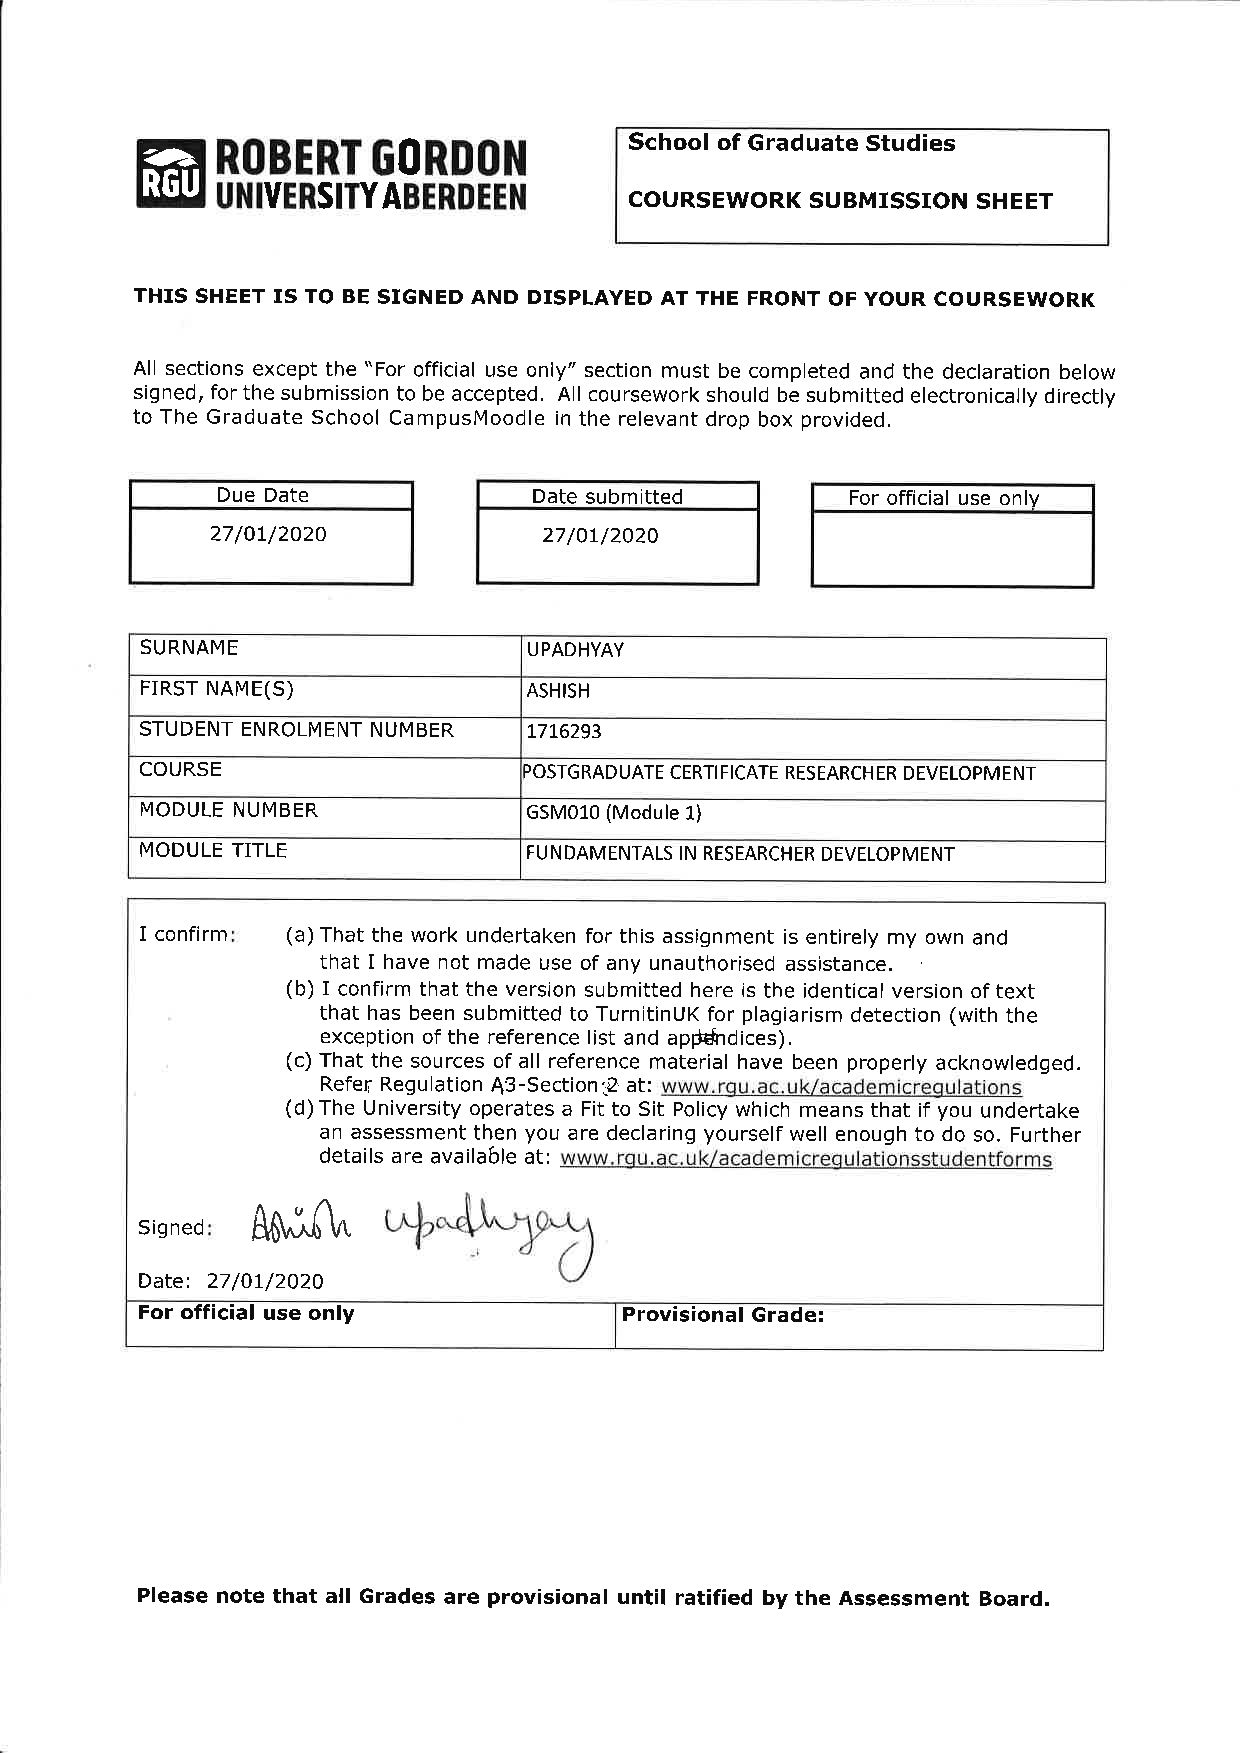
\includepdf{misc/cover_signed.pdf}

\title{Machine/Deep Learning based Performance Enhancement of Natural Language Processing in Business Processes}
\author{
Ashish Upadhyay (a.upadhyay@rgu.ac.uk) \\ 
\textbf{Principle Supervisor}: Dr. Stewart Massie (s.massie@rgu.ac.uk)}
\date{}
\maketitle 

\makeatletter
\renewenvironment{abstract}{%
    \if@twocolumn
      \section*{\abstractname}%
    \else %% <- here I've removed \small
      \begin{center}%
        {\bfseries \Large\abstractname\vspace{\z@}}%  %% <- here I've added \Large
      \end{center}%
      \quotation
    \fi}
    {\if@twocolumn\else\endquotation\fi}
\makeatother

\begin{abstract}

With the evolution of web and cloud computing the amount of data generated is higher than ever. Most of the data is in unstructured textual format. The generated data can help many industries automate their everyday business processes by analysing and processing them. There is a strong need for the development of effective approaches that can process the natural language automatically. Initial solutions to these problems were applying custom rule-based approaches that can be very specific to the problem domains. They require a lot of domain expertise for crafting the features and the performance with these methods was also poor. New approaches employed with machine and deep learning methods for solving the natural language related tasks has given a huge performance gain in the literature due to their ability to learn from the previous data. But the methods proposed in academic research often fail when implemented in real-world applications due to the difference in nature of problem in business processes. One of the drawbacks can be the requirement of a lot of labelled data for training the learning models as in the business processes the labelled data is generated as the part of the process.

In this research we will identify these kind of problems faced by business process during the implementation of current state-of-the-art methods and help them improve their natural language processing performance employed with machine/deep learning. We expect our research contributions to be in the area of business process automation with focus on machine and deep learning. Importantly this work will develop novel algorithms and possibly some dataset which will be made available in public doamin with the aim of helping industries with less resources to enhance their everyday business process.

\end{abstract} 
\clearpage

\tableofcontents
\clearpage

% \listoffigures
% \clearpage

% \listoftables 
% \clearpage

\section{Introduction}
The evolution of the Web combined with the emergence of cloud computing has led to an enormous growth in the amounts of data and information available for organisations to employ in their business processes. The statistics suggest 80\% of business-relevant information originates in unstructured form, typically text; the volume of generated data is growing with predictions that by 2023, we’ll be sending over 350 billion emails daily \cite{email_site}. These statistics make a strong case for the development of effective approaches for natural language processing. 

Sentiment analysis is on area of natural language processing that has delivered good performance, largely due to the general nature of the challenge \cite{sun2019fine,yang2019xlnet}. Effective solutions have been developed, initially employing lexicon-based approaches \cite{mukras2007selecting}, but more recently supplemented with Machine Learning and Deep Learning approaches \cite{devlin2018bert}. Solutions have become more refined in looking at aspect-based sentiment analysis \cite{bandhakavi2018context} and more fine grained in looking at emotion analysis \cite{bandhakavi2017lexicon}. As a result of the improved performance from these developments, sentiment analysis is now a commonplace approach employed by industry. 

The challenges is to develop approaches that go beyond sentiment analysis and to develop NLP solutions supporting business processes more generally \cite{budek_2019}. One on-going requirement is to support the extraction of actionable knowledge from text for custom business processes \cite{Bordignon2018bpm}. Custom rule-based solutions have been developed that typically fill out slots in predefined templates. But these methods lack in giving good performance as well as they are too domain specific. By just changing the problem domain, similar kind of problems can not be solved with the same approach. In this project we hope to develop machine and deep learning based approaches that can outperform the custom rule-based solutions and make similar performance gains that has been seen recently in sentiment analysis. 

There are many business processes that require NLP solutions like document classification, text generation/summarisation, or knowledge extraction as part of the operation workflow e.g. risk assessment, compliance management, auditing, recruitment, and procurement \cite{Sintoris2017bpm}. In many industries, compliance management involve use of a large number of regulatory documents from different statutory bodies at various scenarios. The possible problems statements can be: sorting and prioritizing the documents based on their source organisation, e.g., HSE, BSI; each regulatory document may contain a large number of compliance requirement (CR) that needs to be identified and extracted; after extraction the CR needs to classified by importance and assigned to different job roles. 

There are multiple challenges in relation to these problem statements;

% In this project the intention is to give a clear focus by initially concentrating on one problem. In the recent OGIC funded project at CSDM School, developing a compliance management system has identified a suitable use case. It has become apparent that the state-of-the-art is not yet sufficiently developed to provide an effective practical solution for the extraction of compliance requirements from regulatory documents.


\begin{itemize}
    \item NLP techniques can struggle when they encounter proprietary formats, such as pdf, because the structure of the document on which approaches may rely is lost.
    \item Automated business processes are expected to perform with extremely high accuracy in order to eliminate the manual intervention. Employing feedback loops is one approach to improving accuracy but are expensive to embed in rule-based techniques.
    \item Business processes may have unbalanced cost of error. For example, in case of CR extraction the focus is on minimising the false positives.
\end{itemize}

There are alternative use cases, e.g. assessing applicants’ suitability for a job from analysis of CVs. For a company getting hundreds or thousands of applications for some job roles, it would very difficult for them to hire a lot of experts in order to scrutinize the CVs. It would be very helpful for such company if an automated system is developed capable of filtering these CVs and selecting suitable candidates for further processes. The alternative use cases share similar kind of challenges.

Machine and Deep learning approaches can address the above challenges but rely on availability of labelled data, which is expensive to acquire. Business processes get labelled data as a part of their process. It is not feasible to wait for a long amount of time to get enough labelled data for supervised training. We need to build systems which are reliable with less training data as well. This scenario is referred as cold start problem where we have very minimal labelled to start with and as time goes on the labelled data builds up gradually as well.

The rest of the paper is organised as follows: in chapter \ref{sec:rq}, we talk about the research question and the objectives we hope to meet in order to answer the question; in chapter \ref{sec:lit_rev}, we review the literature and talk about different tasks and methods in natural language processing; in the next chapter \ref{sec:methods}, we present our methodology that we hope to adopt in order to meet our objectives followed by some initial work in chapter \ref{sec:initial_work} and identified impact in chapter \ref{sec:impact}. Finally in chapter \ref{sec:time_plan}, we conclude the paper with time management plan for next three years of the PhD.
% \clearpage

\section{Research Questions and Objectives}\label{sec:rq}
This research will explore the problems involved in text mining in a business process with the goal of improving performance of current state-of-the-art performance. The primary research question for this project will be:
% a goal of developing better system capable of increasing the current performance.
% aim towards developing the a system capable of extracting knowledge from text and mapping that information to a specific business requirement.

\vspace{12pt}

\noindent \textbf{Can Machine Learning help improve the performance of natural language processing related problems in business processes?}

\vspace{12pt}
% \noindent 
Business processes use different automated systems to solve the NLP related tasks. They mostly use the state-of-the-art methods proposed by academic research which is not always enough as the environment where academic research is conducted is different from the real-world scenario of a business process. We hope to meet following objectives in order to answer the research question.

\paragraph{Objectives}\label{sec:objectives}

\begin{itemize}

    \item[\textbf{O1}] Identifying the NLP related problems in business processes that are not well addressed by academic research.
    % research gaps in literature when applying text mining to business processes.
    % Identifying the problems in business processes with respect to text mining that are not addressed in general academic research.
    \begin{itemize}
        % \item[-] What are the problems that arise while implementing literature methods on real-world data in real-time scenario?
        \item[-] Academic research simplifies a real-world problem in order to gain good performance like working with a pre-processed labelled data.
        \item[-] But in a real world scenario, enough labelled data might not be available for training of learning algorithms. The data is generated as a part of the business process.
    \end{itemize}
    
    % in Cold Start Scenario.
    \item[\textbf{O2}] Identifying the common use-cases from business processes and gathering data for those use-cases.
    \begin{itemize}
        % \item[-] What are the most common use cases in business processes in terms of text mining problems.
        \item[-] There are different types of problems related to NLP in business process like natural language generation, text classification, or question answering.
        % \item[-] We 
        \item[-] We will identify some use-cases that are very common throughout the industry.
        \item[-] While selecting the use-case, focus will also be on the availability of datasets.
    \end{itemize}
    
    % Selecting datasets and identifying the use case.
    \item[\textbf{O3}] Setting up the benchmark performance by implementing state-of-the-art algorithms for the real-world scenario.
    \begin{itemize}
        % \item[-] How can we make use of public datasets to simulate a business process scenario in order to test current state-of-the-arts on real world problems.
        \item[-] By using public datasets, we will simulate the real-world scenario to apply the current state-of-the-art algorithms. For example, this can be achieved by applying time stamps on the public datasets. 
        \item[-] This will identify the performance of current state-of-the-art algorithms on real-world scenario.
        % For example, adding timestamps to public datasets 
    \end{itemize}
    
    \item[\textbf{O4}] Developing novel methods to outperform the current state-of-the-art algorithms and evaluating them with real world data on different use-cases.
    \begin{itemize}
        \item[-] After we identify the gaps between business processes and academic research we will propose our algorithms that can enhance the performance of NLP systems in business processes.
        \item[-] We will also evaluate our methods on real-world scenario, if possible, with some industrial data.
    \end{itemize}
    % Proposing novel methods on tackling the problems.
    
    % \item Evaluating the proposed methods in real-world cold start scenario in different use cases.
\end{itemize}


% \begin{itemize}
%     \item [\textbf{O1}] Identify the gap between problems in business process and academic research in terms of natural language processing.
%     \begin{itemize}
%         \item There is a huge difference in the types of problems faced in business process as compared to academic research.
%         \item For example, in a business process the labelled data is generated in streams as a part of the process. Whereas in academic research, we develop solutions for the pre-processed  quality dataset.
%         \item We will identify these kinds of gaps and propose methods to solve them.
%     \end{itemize}
    
%     % \item [\textbf{O2}] Propose the solution for those identified gaps.
%     % \item [O1] Develop novel deep learning algorithms that can improve the performance of text mining in business process. 
    
%     \item [\textbf{O2}] Develop novel techniques to handle the textual data in cold start scenario for business process.
%     \begin{itemize}
%         \item Cold start is one of the gaps between business process and academia.
%         \item Either we have small amount of labelled data or huge amount of unlabelled data to start with.
%         \item We will develop novel techniques to handle this scenario.
%     \end{itemize}
%     % \item [O3] Develop the mechanism for retraining the model on original data instead of synthetic data after an interval.
% \end{itemize}

% \clearpage

\section{Literature Review}\label{sec:lit_rev}
Natural Language Processing (NLP) has come a long way from the era of batch processing and punch cards where a sentence analysis query used to take almost seven minutes to the era of search engines like Google and Bing where millions of web pages are crawled within seconds to produce the best results \cite{Cambria2014}. NLP is a way for computers to perform natural language related tasks like information extraction (like POS tagging, Named Entity Extraction) or language generation and summarisation (like machine translation, dialogue systems) \cite{Young2018}.

% There are different types of tasks in NLP guiding the research in this domain ranging from lower level problems like NER and POS tagging to higher level problems like machine translation and question answering. 
In the next \cref{sec:tasks}, we briefly discuss the various tasks of NLP on different levels. To solve these tasks, there are various methods in the literature which we broadly divide into two categories; Knowledge Engineering (\cref{sec:ke}) and Representation Learning (or in common words, deep learning \cref{sec:dl}). Earlier, knowledge engineering approaches were use to solve NLP tasks. But problem with these methods is that they rely on domain expertise for engineering the knowledge from data. With the development and success of deep learning methods in vision tasks, deep learning has been employed for NLP tasks as well and has been successful as well. The benefit of these methods is that they do not need any special knowledge engineering as they automatically learn features modelling the data during their training phase. This learning is iteratively updated in various steps during training.
% The main difference between two is that the former requires a lot of feature engineering whereas the later automates the process of feature extraction using dense representation of text. 
% In the final \cref{sec:initial_work}, we will take a real world example using the compliance data from Oil and Gas industry and evaluate these methods.

% The techniques present in literature for solving these tasks. We will briefly discuss about how the fields of industry and academia differ in taking to approaches to the solution for these tasks.

% Solving these NLP tasks were a real hassle for a long time. They required an extensive need of domain expertise in order to derive some knowledge that will suit for a given problem. But with the advancement of deep learning in the field of NLP we have got new solutions that are not specific to the domain of the problem. Same method can be applied to different problems from different domains with very little fine tuning with respect to domain specific data.

% The breakthroughs in academic research take a long time to be implemented in the industry. This is due to problem of available labelled data-set for training the 

% Here we can broadly divide the problem solving approaches into two categories: knowledge engineering and deep learning. 


% \section{Background on NLP}
\subsection{Tasks}\label{sec:tasks}
NLP research is mostly driven by the basic question, how do humans understand the natural language and how can we make the machines do the same? In the research, understanding the natural language for machines differs from lower level problems of extracting information from the text like named entity or relation extraction to higher level problems like machine translation or question answering. In this section we will discuss about the different kind of tasks involved in NLP dividing them into three broad categories:

\begin{enumerate}
    \item Extraction
    \item Generation
    \item Summarisation
\end{enumerate}

\subsubsection{Extraction}
Knowledge Extraction is a sub field of NLP that deals with the automated extraction of structured knowledge from unstructured sources. These are the few examples of the tasks that can be treated as knowledge extraction.

\paragraph{Named Entity Recognition}
Named Entity Recognition is the a sub task of Knowledge Extraction that deals with identifying the various entities in a piece of text such as person, location, organization and date. It has various use cases, like automating hiring process or optimizing the search engine algorithms. One of the main approach is to use BIO notation (B for beginning, I for inside and O for non-entity tokens.) For example, in the sentence \textit{`Boris Johnson won the UK general elections'} the entities can be marked as $[Boris]_{B-PER}$ $[Johnson]_{I-PER}$ $[won]_{O}$ $[the]_{O}$ $[UK]_{LOC}$ $[general]_{O}$ $[elections]_{O}$. PER represents person, LOC represents location and O is the non-entity tokens.

There are various open source libraries for NER such as spaCy which uses hand crafted features (not published) and StanfordNLP which uses a combination of hand crafted features and deep learning for the same task. One of the most popular benchmark for NER is CoNLL 2003 \cite{sang2003introduction} consisting text from news wires like Reuters dataset tagged in four different categories (PER, LOC, ORG, MISC). The state-of-the-arts in literature for NER right now are mostly based on the transformers architecture which we will discuss is \cref{sec:transformers}

% NER SRL Chunking sequence tagging
% Named Entity Recognition deals with 

\paragraph{Parts-of-Speech Tagging}
deals with the marking of parts of speech of a word in the text corpus. The category of words having similar grammatical properties can be termed as parts-of-speech. Some of the common parts-of-speech in English language are noun, pronoun, adjective, preposition, verb, adverb etc. NLTK is one of the most common open-sourced library used for POS tagging. A example of POS tagging in NLTK for the sentence \textit{`And now for something completely different'} can be \textit{[('And', 'CC'), ('now', 'RB'), ('for', 'IN'), ('something', 'NN'),
('completely', 'RB'), ('different', 'JJ')]}. Here CC is coordinating conjunction, RB is used for adverbs, IN is a preposition, NN is noun and JJ is adjective \footnote{Example taken from \url{https://www.nltk.org/}}.

The popular benchmarks for POS tagging are Penn Treebank \cite{marcus1993building} and Universal Dependencies \cite{silveira14gold}. Penn Treebank portion of Wall Street Journal (WSJ) consists of 45 different POS tags whereas Universal Dependencies consists of more than 100 treebanks from 60 different languages. The current state-of-the-arts for POS tagging are mostly based on LSTM and BERT.

\paragraph{Natural Language Inference}
For a given piece of text or premise, finding that whether some `hypothesis' about that text is true or not is called natural language inference. If a hypothesis is true then it is known as `entailment', if it is false then `contradiction' and for undetermined `neutral'. For example, lets have a look at the \cref{tab:nli} \footnote{Example taken from \url{https://nlpprogress.com/}}.

\begin{table}[h!]
  \begin{center}
    \caption{NLI Example}
    \label{tab:nli}
    \begin{tabular}{l|c|r} % <-- Alignments: 1st column left, 2nd middle and 3rd right, with vertical lines in between
      \textbf{Premise} & \textbf{Label} & \textbf{Hypothesis}\\
      \hline
      A man inspects the uniform of a & contradiction & The man is sleeping.\\
      figure in some East Asian country. &  & 
    \end{tabular}
  \end{center}
\end{table}

The two most common corpus for NLI are Multi-Genre Natural Language Inference (Multi-NLI) \cite{williams2017broad} and Stanford Natural Language Inference (SNLI) \cite{bowman2015large}. Both of them contain around 500k labelled hypothesis/premise pairs. Current state of the arts are based on the slight modification of BERT architecture.

\paragraph{Relation Extraction}
The task of identifying semantic relationships between entities of text is known as relation extraction. Usually the relations are defined between two or more entities like person, location or organisation and fall under various pre-defined semantic categories.

There are lots of public datasets available for relation extraction and all of them define their own category of relations that need to be extracted from the text. Few examples are; Capturing discriminative attributes (SemEval 2018 Task 10) \cite{krebs2018semeval} where users are asked to identify if a given attribute can help in discrimination between two concepts. Few-Shot Relation Classifier (FewRel) \cite{han2018fewrel} consisting of 70k sentences with 100 different kinds of relation annotated by crowd-sourcing on wikipedia corpus. New York Times corpus \cite{riedel2010modeling} containing entities extracted from NYT corpus and linked to the freebase knowledge base. 
% There are different types of state-of-the-arts based on hand crafted features as well machine/deep learning algorithms to achieve good results on these datasets.

% \paragraph{Template Filling} The approach of efficient extraction and representation of 

% \paragraph{Semantic Role Labelling}


% \paragraph{Dependency Parsing}

\subsubsection{Generation}
Natural Language Generation (NLG) can be termed as the sub-field of NLP which deals with the generation of natural language given some structured or unstructured information. Machine Translation and Data Augmentation can be few examples of NLG.

\paragraph{Machine Translation}
Machine Translation has been one of the most popular problems in NLP. It deals with the translation of text from one natural language to another, for example, translating English text to Hindi or vice-versa. A snippet from Google translate performing MT is shown in fig. \ref{fig:mt_example} \footnote{\url{https://translate.google.com/}}.

\begin{figure}
    \centering
    
\includegraphics[width=\textwidth]{images/mt.png}
    \caption{An Example of Machine Translation}
    \label{fig:mt_example}
\end{figure}

The MT models are evaluated on the method called BLEU score which is used as the higher the better. Some of the common public datasets availabel are WMT 2014 EN-DE and WMT 2014 EN-FR \cite{bojar-EtAl:2014:W14-33} which contains many english-german and english-french pair of sentences. The current state-of-the-arts are based on mainly transformers and some attention based LSTMs.

\paragraph{Data Augmentation}
With the popularity of Deep Learning based NLP, there has been a huge requirement of training data for building the models. Collecting the labelled data is sometime very costly and take a lot of resource in terms of time and money. 

The alternative way of getting more data is to generate a huge corpus of data by tweaking the using the small amount of training data available in some fashion. This technique is known as data augmentation. The way of tweaking differs from problem to problem. There are different ways of data augmentation like unsupervised back translation with consistency training \cite{Xie2019} or contextualized word replacement \cite{kobayashi2018contextual}.

\subsubsection{Summarisation}
The third category of NLP tasks is termed as the problem of summarisation. Given a piece of text, how can we summarize the information it posses in simpler and/or structured manner. 

\paragraph{Text Classification}
Classifying a piece of text/document into some pre-defined categories can be termed as the task of text classification. Text classification is mainly used in applications like sentiment analysis and/or topic and document classification. 

For example, in sentiment analysis we try to identify the sentiment or polarity of a sentence based on its content. Given a review about a product on Amazon and identifying if the customer who wrote the review is positive or negative about the product's quality. Some of the common examples for topic classification can be identifying the domain (political, religious or technological) of a news article based on its content.

Some popular datasets for sentiment analysis are; imdb movie reviews which contains 50,000 reviews of different movies from imdb website labelled into positive and negative classes. They also contain a numeric value from 1 to 10, 1 being the lowest rating and 10 being the highest rating. The current state-of-the-art is XLNet based on the transformer architecture for this \cite{yang2019xlnet} dataset.

Another famous dataset for text classification is Dbpedia dataset which consist of 5.6M labelled texts from the 14 non-overlapping topics of wikipedia. BERT \cite{devlin2018bert} is the current best performing algorithm with only 0.64 error rate on this dataset.

\paragraph{Question Answering}
Question Answering is a token-level task of NLP where given a piece of information with some question related to it, the system needs to generate an acceptable answer for it. One of the most famous dataset for this task is Stanford's Question Answering Dataset (or SQuAD) which consists of different questions asked by users of wikipedia related to some wikipedia article. The answer to this question is a segment from the same article only. The current state-of-the-arts for this datasets are the ensemble models based on different versions of BERT. An updated leaderboard for this dataset can be found on their website \footnote{\url{https://rajpurkar.github.io/SQuAD-explorer/}}.

% \paragraph{Aspect-Based Sentiment Analysis}

% \paragraph{Summary Generation}
% Chat-bots in NLP are very popular in today's world. They can interact with the users in a very humane manner and are very efficient. Suppose, a company has to interact with their customers on the website on the daily basis. One way to answer the queries of these customers will be have support assistants hired to answer these queries as the part of their job. But this can be very expensive. On the other hand, the company can use an automated software to do the same job if 

\subsection{Knowledge Engineering}\label{sec:ke}
Initially, the solutions for NLP problems were all based on a common approach of identifying better features to represent the text data. These features are identified based on the domain expertise and are very specific to the problem they are applied in. This category of techniques can be classified as the techniques which requires a lot of domain knowledge in order to achieve good results. They don't need a lot of training data in order to gain good performance but the performance gets saturated after some amount of data, i.e., the performance doesn't increase with the increase in training data. We group these methods into two categories:

\begin{enumerate}
    % \item Rule Based
    \item Case Based Reasoning
    \item Machine Learning
\end{enumerate}

% \subsubsection{Rule Based}
% The techniques which requires a pre-defined set of rules to identify the matches and solve the problem.

% \paragraph{Syntax driven} It takes a syntax driven approach to semantic 

% is the approach where syntax

% \paragraph{Lexicon approach} requires a set of dictionary/lexicon defined in order to identify 

% \paragraph{Ontology based}

% \paragraph{Linguistic Features}\label{sec:ling_ftrs}
% A sentence can be processed to extract parts of speech, noun chunks, and entities. Some of the features that can be generated afterwards are as follows:

% \begin{enumerate}
%     \item word length: number of tokens in sentence.
%     \item word length 2: number of words in sentences with stopwords removed.
%     \item has modal: indicates if the sentence contains a modal.
%     \item num of modals: number of modals in sentence.
%     \item modal position: average position of modal verbs in a sentence (-1 if none).
%     \item num of entities: number of named entities in sentence.
%     \item m trigger word: checks if the sentence contains any mandatory term (true/false).
%     \item m trigger position: average position of mandatory terms in sentence ([0.0,1.0] interval and -1 if none).
%     \item n trigger word: checks if the sentence contains any non-mandatory term (true/false).
%     \item n trigger position: average position of non-mandatory terms in sentence ([0.0,1.0] interval and -1 if none).
% \end{enumerate}


\subsubsection{Case Based Reasoning}
Case Based Reasoning is a sub-field of Artificial Intelligence which solves the problems on the basis of modelling real word intuition that similar problem have similar solutions. When we see a new problem in our real life, we try to map it to our previous experience of similar problems and solve it taking similar approach. In CBR as well, we retrieve the problems similar to the new one and use the similar kind of approach to solve it using the solutions stored in knowledge base (KB). In the KB, we store these cases in a pair of problem and solution. A CBR cycle generally have 4 steps as defined in \cite{aamodt1994case}. Fig. \ref{fig:cbr_4r} shows the 4Rs of a CBR cycle.

\begin{enumerate}
    \item RETRIEVE the cases similar to the new problem.
    \item REUSE the information or solution for similar cases to solve the new one.
    \item REVISE the new proposed solution.
    \item RETAIN the useful information of new case in the KB for future use.
\end{enumerate}

\begin{figure}
    \centering
    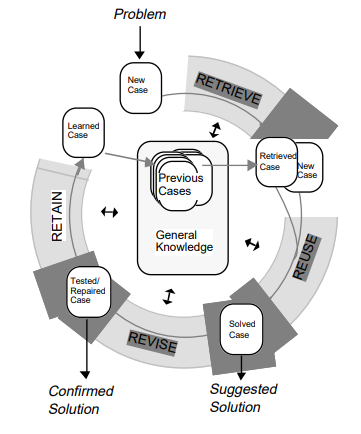
\includegraphics[width=0.45\textwidth]{images/cbr_4r.png}
    \caption{4Rs of a CBR Cycle \cite{aamodt1994case}}
    \label{fig:cbr_4r}
\end{figure}

\paragraph{k-Nearest Neighbours (k-NN)} One of the most common CBR algorithm is k-Nearest Neighbour which computes the distance between the new case and all other previous cases. Then the k cases with the minimum distance are selected as the similar cases and there solution is used to make decision for the new case's solution. k-NN uses the euclidean distance to measure distance between two cases. The distance between two cases $c_{i}$ and $c_{j}$ is given in \cref{eq:knn}

\begin{equation}
    \label{eq:knn}
        Dist(c_{i}, c_{j}) = \sqrt{\sum_{v=1}^{n} (c_{iv}-c_{jv})_{2}}
\end{equation}

where v is the dimension of problem in the case. This technique is also referred as lazy learning sometimes as it makes observation on the previous knowledge every time a new query is given rather than trying to learn a general model for knowledge base in training and using that model to answer a query when asked.

\paragraph{Textual Case-Baed Reasoning (TCBR)}
TCBR is a bit different from general CBR in terms of representation of problem and solution of the cases, altough the 4Rs of a CBR cycle holds true here as well. In TCBR, some or whole part of the previous cases are stored in textual form and we aim to solve the problem for new cases with the help of these textual knowledge sources in automated way \cite{weber2005textual}. The cases are stored in two sets namely, problem set and solution set. In TCBR, the focus is on defining a good representation of these sets and then finding a way to evaluate these representations.

\paragraph{Text Representation}
Representing cases in text CBR is a trivial task as there is no standard representation defined that can work for every problem. But one of the most commonly used representation is using bag of words \cite{10.5555/646268.684025}. In this representation, a sentence is is broken into tokens which are essentially the words of the sentence and their appearance is different manner is used as the features. One of the drawback of using this technique is that we loose the sequence information as it is lost during the tokenisation process.

Another common way of representing texts is by grouping them into attribute-value pairs to generate feature vectors, where attributes are decided based on the domain and values are the pieces of text from the case base. This approach works for maximum cases but the attributes differ from problem to problem as they are domain specific. An example of attribute-value pair can be a case storing the information of a student with attributes such as \textit{Student Name - Ashish Upadhyay} and \textit{School - Computing Science and Digital Media}.

There are other examples of case representation as well, like used in popular CBR framework jCOLIBRI where cases are stored in tree structure where each case is treated as an individual capable of containing other individuals and thus forming the tree structure.

\paragraph{Evaluation}
After the representation of text cases is done, we need to evaluate it by measuring the similarity or alignment between cases problem and solution set. A good representation will provide much better alignment between cases than a bad representation.

Two most common ways of measuring the similarity can be local alignment and global alignment \cite{raghunandan2008evaluation}. The local alignment measure uses the alignment of each case with its neighbourhood and then aggregates the values for all cases to find the alignment for whole case base whereas the global method measures the alignment value for whole case base as one single entity.

\subsubsection{Machine Learning}
Machine Learning is another subset of Artificial Intelligence which learns a general distribution of the previous experience by using the training data and then uses the learned distribution to predict the answer a new problem. In Machine Learning, we mostly use sparse representation of the problems of a case and use statistical algorithms to learn the general distribution of training set.

The difference of machine learning approach from case-based approach is that machine learning, the distribution is learned during the training process and that learning is used to answer a query during test or deployment phase whereas in case-based reasoning, the case-base is searched to retrieve the similar cases every time a query is asked in order to answer it.

Some of the representations and learning algorithms used in machine learning are briefly discussed here. Term Frequency (TF), Term Frequency-Inverse Document Frequency (TFIDF) and Linguistic Features are some of the most common feature representations, whereas Support Vector Machines, Random Forest and Naive Bayes are some of the commonly used learning algorithms.

\paragraph{Term Frequency Vectors}
This feature vector is used to represent a document by assembling a vector of the frequency of the terms contained in the document. Here we first extract all the terms from the  documents and  create a corpus dictionary of all the terms. Then the frequency of  the terms from each document is calculated to generate the vector representing that document. The vectors can be presented as a document term matrix, where each row  is a document vector and each column represent a term from the corpus dictionary.

To calculate the term frequency we apply the following formula: 
\begin{equation}
tf(t) = m/k
\end{equation}
Where, the number of times term $t$ has appeared in a document is represented by $m$ and the total number of terms in the document is denoted by $k$.

Let's understand this with an example. Suppose, in our training dataset we have $N$ documents. After extracting all the terms from the documents and creating the corpus, we get total $M$ unique terms. So our count vector will be a $N\times M$ matrix where every row is a document and every column is a term from the corpus. So each document is represented as a $1\times M$ vector.

For example, let's say we have two documents:
\begin{center}
	D1: The valve must be coloured black.\\
	D2: The wire must remain covered.
\end{center}
Thus the corpus dictionary created would look like this:
\begin{center}
	[`be', `black', `coloured', `covered', `must', `remain', `the', `valve', `wire']
\end{center}
So, the count vector for this example would be a $2\times 10$ matrix and can be represented as follows:
\begin{table}
	\centering
	\caption{TF vector representation.}\label{tab2}
	\begin{tabular}{|l|l|l|l|l|l|l|l|l|}
		\hline
		be & black & coloured & covered & must & remain & the & valve & wire\\
		\hline
		0.166 & 0.166 & 0.166 & 0 & 0.166 & 0 & 0.166 & 0.166 & 0\\
		0 & 0 & 0 & 0.166 & 0.166 & 0.166 & 0.166 & 0 & 0.166\\
		\hline
	\end{tabular}
\end{table}


\paragraph{Term Frequency - Inverse Document Frequency Vector}\label{sec:tfidf}
This feature vector is different from the TF vector in a way where it takes into account the occurrence of a term in whole corpus not just the occurrence of that term in a document. The intuition behind this is to reflect how important a term is to document by giving popular terms a low weight and rare terms a higher weight. The TF-IDF can be divided into two parts: term frequency and inverse document frequency. 

For calculating term frequency, we can use the same method discussed above in Equation 1.

Then we calculate the inverse document frequency by using the following formula.
\begin{equation}
idf(t) = log(N/n)
\end{equation}

Where $n$ is the number of documents term $t$ has appeared and $N$ is the number of documents.

So, the formula to calculate $tfidf$ is given as:
\begin{equation}
tfidf(t) = tf*idf = (m/k)*\log(N/n)
\end{equation}

That's why in this way,  terms like $the, is, a$ are heavily penalized.  Rarely occurring terms in a corpus get high $idf$ score. To compare with the TF representation, let's take the same example discussed in previous section. So, the $tfidf$ for term $the$ from document $D1$ can be calculated as:
\begin{center}
	$tf = 2/8 = 0.25$\\
	$idf = \log(2/2) = 0$\\
	$tfidf = 0.25*0 = 0$
\end{center}

\paragraph{Linguistic Features}\label{sec:ling_ftrs}
A sentence can be processed to extract parts of speech, noun chunks, and entities. Some of the features that can be generated afterwards are as follows:

\begin{enumerate}
    \item word length: number of tokens in sentence.
    \item word length 2: number of words in sentences with stopwords removed.
    \item has modal: indicates if the sentence contains a modal.
    \item num of modals: number of modals in sentence.
    \item modal position: average position of modal verbs in a sentence (-1 if none).
    \item num of entities: number of named entities in sentence.
    % \item m trigger word: checks if the sentence contains any mandatory term (true/false).
    % \item m trigger position: average position of mandatory terms in sentence ([0.0,1.0] interval and -1 if none).
    % \item n trigger word: checks if the sentence contains any non-mandatory term (true/false).
    % \item n trigger position: average position of non-mandatory terms in sentence ([0.0,1.0] interval and -1 if none).
\end{enumerate}

\paragraph{Random Forest}
Random forest \cite{breiman2001random} is an ensemble algorithm of both multiple decision trees used for classification or regression. It initialises a forest of many random decision trees by applying sampling on the train data. Every tree initialised in the forest uses subset or the random samples of number of observations available as well as only taking the random sample of features from the dataset.

% Suppose, you have a dataset of $n$ observations and $k$ features, i.e., a matrix of $n\times k$ for training and you wish to grow 100 trees in your forest, then every tree in the forest will take random $n_0$ observations and $k_0$ features for training where $n_0 < n$ and $k_0 < k$.

\paragraph{Support Vector Machine}\label{svm}
A Support Vector Machine (SVM) formally defined by a separating hyperplane is a discriminative classifier that can be used to classify both linear and non-linear data \cite{vapnik2013nature}. A Support Vector Machine gives an optimal hyperplane dividing the training examples into different classes. For a multi-class classification where number of classes is more than two, an SVM iteratively finds the optimal plane by diving the problem into one-vs-all. In every iteration, it takes one class as positive and rest of the classes as negative and finds the hyperplane dividing that data combination. SVM can be very slow for large datasets as the time complexity is proportional to the square of features used.

\paragraph{Naive Bayes}
Naive Bayes is an algorithm based on Bayes theorem which models the distribution of a class using independent conditional probability \cite{han2011data}. It is very fast and scalable and can be applied to various problems with bigger datasets in text mining.



\subsection{Representation Learning}\label{sec:dl}
Representation Learning or in common words Deep learning can be considered as a subset of machine learning but has gained attention as a different field due to its success in various vision, text and speech tasks. The difference about deep learning that makes it perform better on various complex problems is that it doesn't require domain expertise to identify the features to represent a problem or case from previous experience. Instead it automatically learns the features during training process using a large set of training data on various iterations. 

Initially deep learning outperformed a lot of state-of-the-art algorithms in vision tasks and established itself as the benchmark solutions \cite{simonyan2014very,he2016deep}, but during the past few years with the advancement in computing powers and the availability of large datasets the \textbf{``The Deep Learning Tsunami''} \cite{manning2015computational} has taken over NLP as well. In this section we will sequentially talk about the development of deep learning applied in NLP to solve the various tasks.

\subsubsection{Word Embeddings} \label{sec:word_emb}
When using deep learning and to solve an NLP task, each word in the vocabulary is represented in a vector form so that it can be fed into the neural networks. Word embedding is the way of converting a word $w_{i}$ in vocabulary $V$ in the form of a vector of $n$ dimensions. These word vectors are generated by unsupervised training on a large corpus of words in order to gain the semantic similarities between the words. Algorithms like word2vec \cite{mikolov2013distributed} and GloVe \cite{pennington2014glove} are used to train these word embeddings. These word embeddings are generally pre-trained and made available to be downloaded from the internet and used directly in the deep learning models.

These distributed representation of words give a certain amount of semantic understanding of the words in a high dimensional vector space. For example, the distance between words $king$ and $queen$ will be similar to the distance between $boy$ and $girl$. In this contrast the \cref{eq:we1} fits perfectly. 
% A visualization of these word embeddings in low dimension is shown in \cref{fig:glove_ex} \footnote{taken from \url{http://web.stanford.edu/class/cs224n/}}.

\begin{equation}\label{eq:we1}
    boy - girl + king = queen
\end{equation}

% \begin{figure}
%     \centering
%     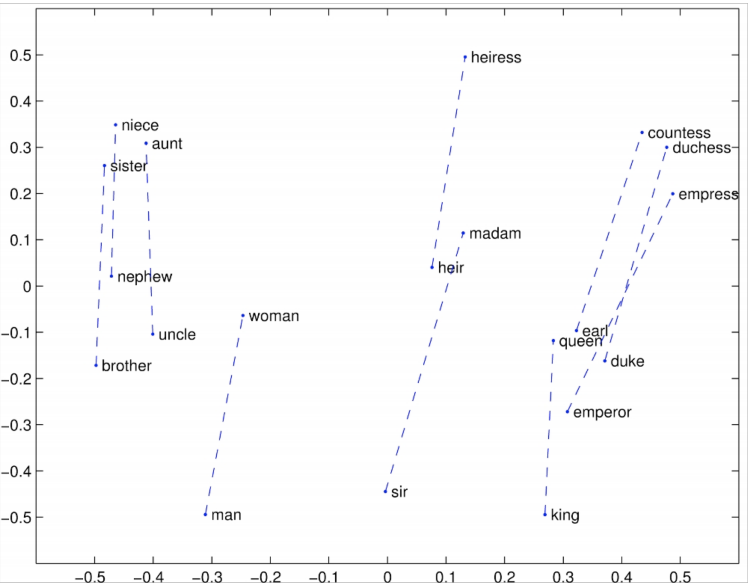
\includegraphics[width=0.5\textwidth]{images/glove_vecs.png}
%     \caption{GloVe words visualization in 2D space}
%     \label{fig:glove_ex}
% \end{figure}

These representations have a drawback that they fail to take context of a word into account. For example, the word \textit{`Scotland'} will have a different meaning in the sentence \textit{`Scotland is one of the most best places to live on earth'} than in the sentence \textit{`Royal Bank of Scotland is one of the top banking firms in the UK'}. The glove or word2vec word embedding will fail to differentiate the two meanings of Scotland and will assign same vector in both the cases. These drawbacks are tackled by a new concept of contextual word embeddings discussed in \cref{sec:context_we}

\subsubsection{Language Models}\label{sec:lm}

\begin{figure}
    \centering
    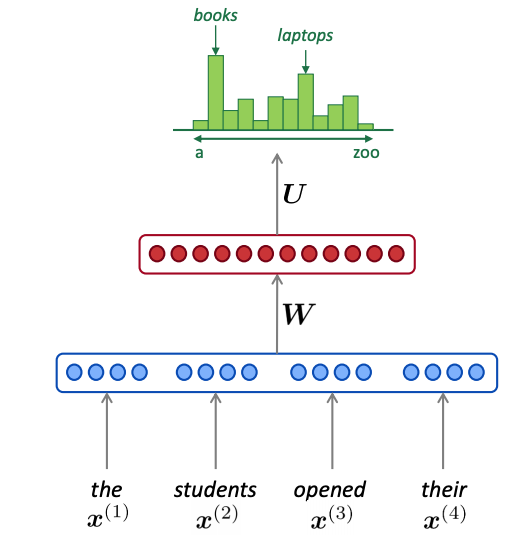
\includegraphics[width=0.45\textwidth]{images/lang_model.png}
    \caption{Prediction of next word using a Language Model}
    \label{fig:lang_model}
\end{figure}

A language model is a type of system that predicts the probability of possible next words given a sequence of words as the input. In general terms, for a given sequence of input $(x_{1}, x_{2}, \cdots, x_{t})$, the probability distribution of next term $x_{t+1}$ is computed from a vocabulary $V$ of $k$ words ($V = (w_{1}, w_{2}, \cdots, w_{k})$). 

\begin{equation}
    \label{eq:lm_dist}
        P(x_{t+1}|x_{1}, \cdots, x_{t})
\end{equation}

Earlier the language models were based on statistical approaches where they used to take a window of $n$ words as a context from the sentence to predict the next word. This approach is also known as $ngram$ Language Model. It takes an simple approach of calculating the conditional probability of next word in the sentence given the window of $n$ words as a context. These $ngram$ probabilities are calculated from counting them in some large corpus of text.

\begin{equation}
    \label{eq:lm_ngram}
        P(x_{t+1}|x_{1}, \cdots, x_{t}) = 
            \frac {P(x_{t+1}, x_{t}, \cdots, x_{t-n+2})} {P(x_{t}, \cdots, x_{t-n+2})}
\end{equation}

or in simpler terms:

\begin{equation}
    \label{eq:lm_count_ngram}
        P(w_{3}|w_{1},w_{2}) = \frac{count(w_{1}, w_{2}, w_{3})}{count(w_{1}, w_{2})}
\end{equation}

This statistical approach has mainly two problems. First sparsity, consider the \cref{eq:lm_count_ngram}, what if $w_{1}$, $w_{2}$ and $w_{3}$ never occurred together. The probability of $w_{3}$ will be 0. Also, if $w_{1}$ and $w_{2}$ then there's no way to calculate the probability of $w_{3}$. Second storage, as we increase the value of $n$, the count of all $nrgams$ we see in the corpus increases as well and so does the need of memory to store them.

The neural language model using Recurrent Neural Networks (\cref{sec:rnn}) were able to model all the words in a sentence without having a need of window to predict the next word at each timestep using hidden state and output from the previous time step combining with the new input at each time step. 


\subsubsection{Recurrent Neural Networks} \label{sec:rnn}
Text is a sequential form of data. To process text and extract information we need a model capable of processing the sequential data. \textit{Recurrent Neural Networks} \cite{elman1990finding} are the most elementary deep learning architectures that are able to learn from sequential data. RNN, are wide in nature as they unroll through time. These networks will have a `memory' component which can store the information about previous state. They share same set of weights throughout the layers, however, will receive a new input at every layer or time-step. The output to every time-step is dependent on the input taken at the current time-step $t_{i}$ as well as the information gained from previous time-step $t_{i-1}$. Specifically, an RN Net will maintain a hidden state $h_{t}$ at every step which is referred as the memory of network. An illustrated diagram of unrolled RNN is shown in fig \cref{fig:rnn_unrolled} \footnote{taken from \url{https://colah.github.io/posts/2015-08-Understanding-LSTMs/}}.

\begin{figure}
    \centering
    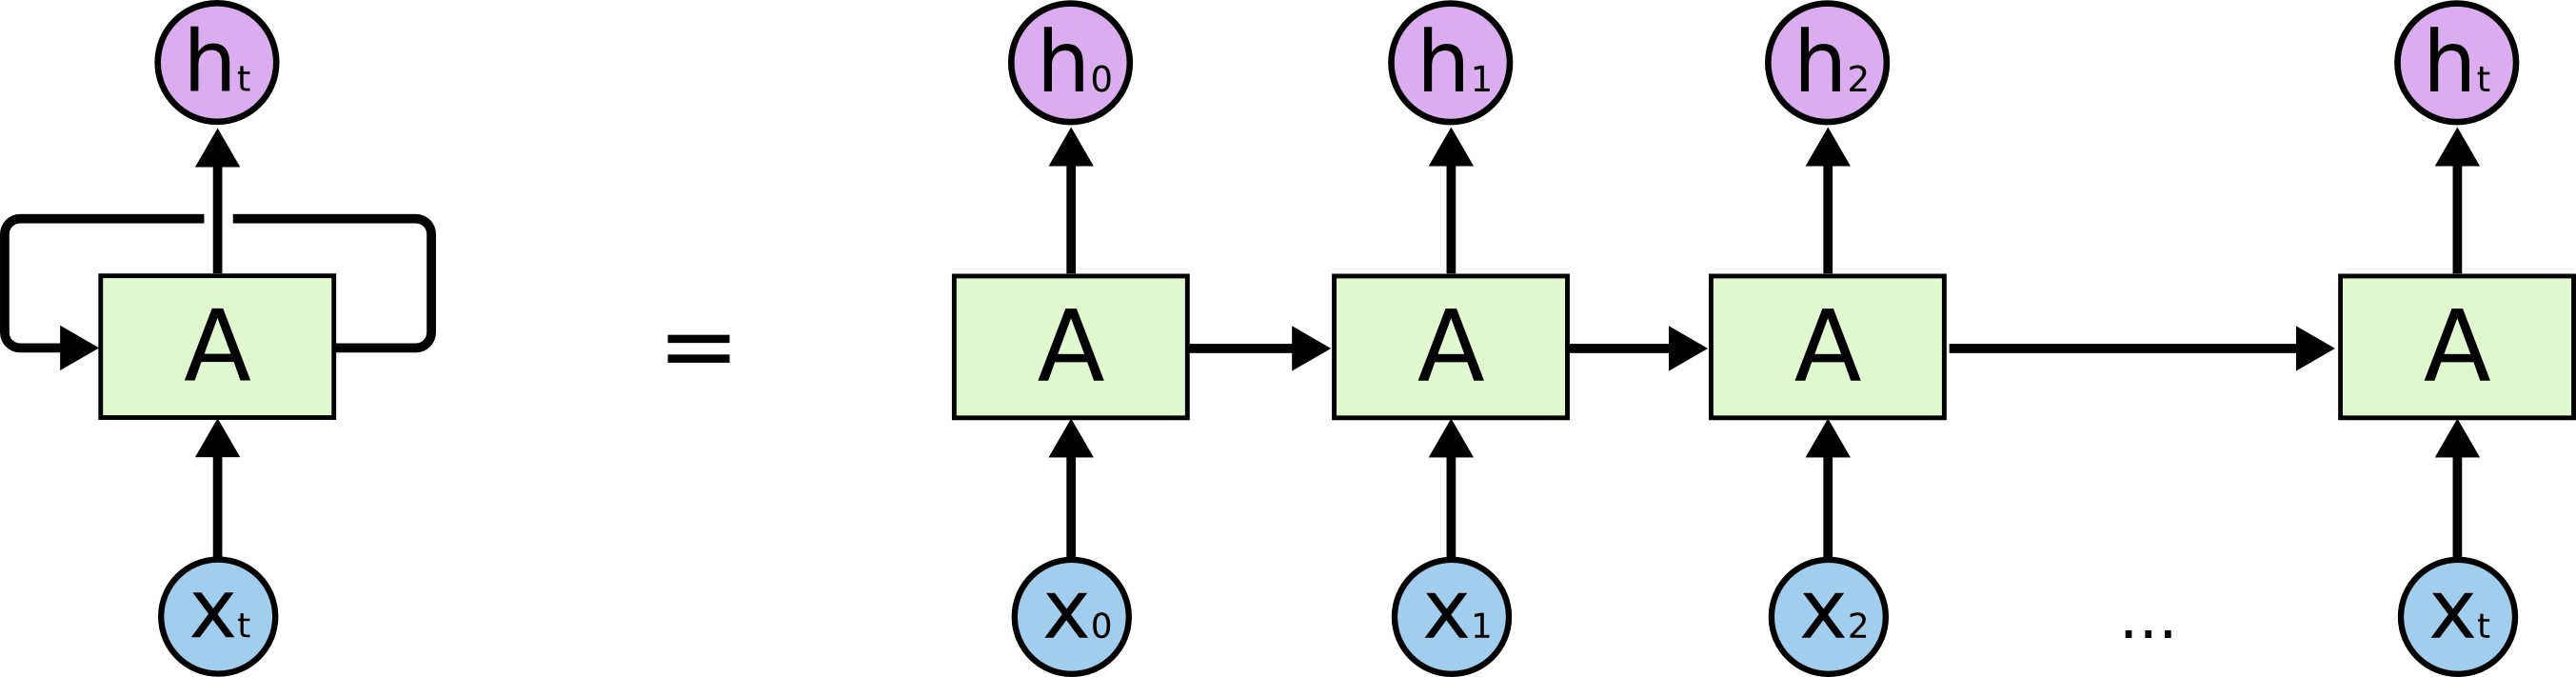
\includegraphics[width=\textwidth]{images/RNN-unrolled.png}
    \caption{RNN Unrolled}
    \label{fig:rnn_unrolled}
\end{figure}

The operations performed in RNN at every time step is given in the \cref{eq:rnn}.

\begin{align}\label{eq:rnn}
    \begin{gathered}
        h_{t} = \sigma_{h}(W_{e}x_{t} + W_{h}h_{t-1} + b_{h}) \\
        y_{t} = \sigma_{y}(W_{y}h_{t} + b_{y})
    \end{gathered}
\end{align}

Here $\sigma_{y}$ and $\sigma_{h}$ are the activation functions. $W_{h}$ is the weight matrix to apply transformation on previous hidden state $h_{t-1}$, $W_{e}$ is the weight matrix to apply transformation on the input $x_{t}$ received over time $t$. Combining these with the bias $b_{h}$ yields hidden state $h_t$ for time $t$. Applying activation on the $h_{t}$ with $W_{y}$ gives the output $y_t$ for every time-step $t$.


\subsubsection{Long Short-Term Memory Networks}
Although, in theory the RNNs are designed to handle the sequence input but in practice they lack in storing the long term dependencies because of the problem of exploding and vanishing gradients \cite{bengio1994learning}. Long Short-Term Memory Networks \cite{hochreiter1997long} are the advanced version of RNNs with a slight modification of being capable of deciding what to `remember' and what to `forget' from the input sequence with the help of a series of gates. LSTM has a number of gates, an output gate, an input gate $i_{t}$, forget gate $f_{t}$, $o_{t}$, all of which are the functions of previous hidden state $h_{t}$ and current input $x_{t}$. These gates interact with the previous cell state $c_{t-1}$, the current input $x_{t}$, and the current cell state $c_{t}$ and enable the model to selectively retain or information from the sequence. The full version of LSTM is given in the \cref{eq:lstm}.

\begin{equation}\label{eq:lstm}
    \begin{gathered}    
        f_{t} = \sigma_{g} (W_{f}x_{t} + U_{f}h_{t-1} + b_{f}) \\
        i_{t} = \sigma_{g} (W_{i}x_{t} + U_{i}h_{t-1} + b_{i}) \\
        o_{t} = \sigma_{g} (W_{o}x_{t} + U_{o}h_{t-1} + b_{o}) \\
        \Tilde{c_{t}} = \sigma_{c} (W_{c}x_{t} + U_{c}h_{t-1} + b_c)\\
        c_{t} = f_{t} \circ c_{t-1} + i_{t} \circ \Tilde{c_{t}}\\
        h_{t} = o_{t} \circ \sigma_{h}(c_{t})
    \end{gathered}
\end{equation}

where $\sigma_{g}$ is the $sigmoid$ activation function, $\sigma_{c}$ and $\sigma_{h}$ are the $tanh$ activation function, and $\circ$ is element-wise multiplication, also known as \textit{`Hadamard product'}. An illustrated diagram of unrolled RNN is shown in fig \cref{fig:lstm} \footnote{taken from \url{https://colah.github.io/posts/2015-08-Understanding-LSTMs/}}.

\begin{figure}
    \centering
    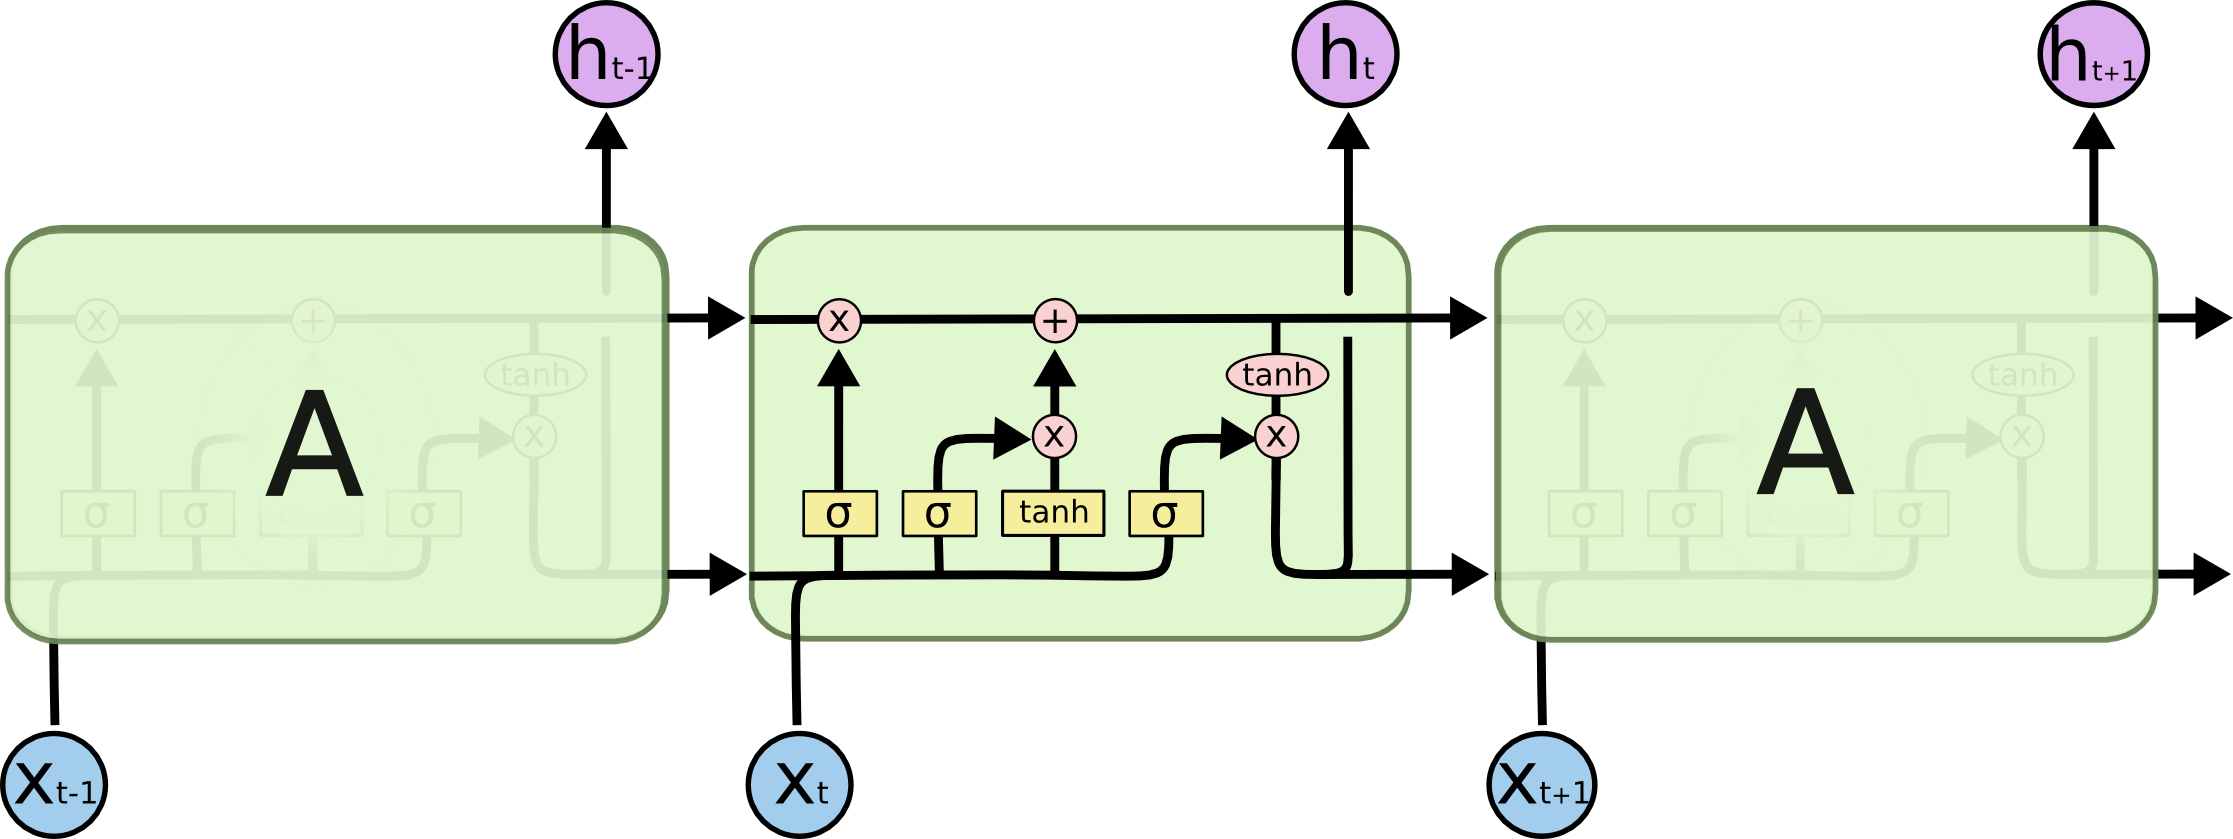
\includegraphics[width=\textwidth]{images/lstm.png}
    \caption{LSTM}
    \label{fig:lstm}
\end{figure}

LSTM layers can be stacked on each other to form multiple layer LSTM architecture. One of the most popular LSTM architecture is Bidirectional LSTM (BiLSTM) \cite{graves2013hybrid}, where two separate LSTMs are ran forward and backward to gain the sequential information in both directions.

\subsubsection{Convolutional Neural Networks}
Convolutional Neural Networks \cite{lecun1998gradient} are the version of deep neural networks established as state-of-the-art in various computer vision tasks \cite{barbu2019objectnet,ali2019mfc}. After the release of AlexNet \cite{krizhevsky2012imagenet} in ImageNet competition 2012, CNNs have been the benchmark for almost every vision task. Inspired from the popularity of CNN in vision, researchers proposed an CNN architecture for sentence classification which outperformed many benchmarks on various text classification dataset ranging from sentiment analysis to topic classification \cite{kim2014convolutional}. 

\begin{figure}
    \centering
    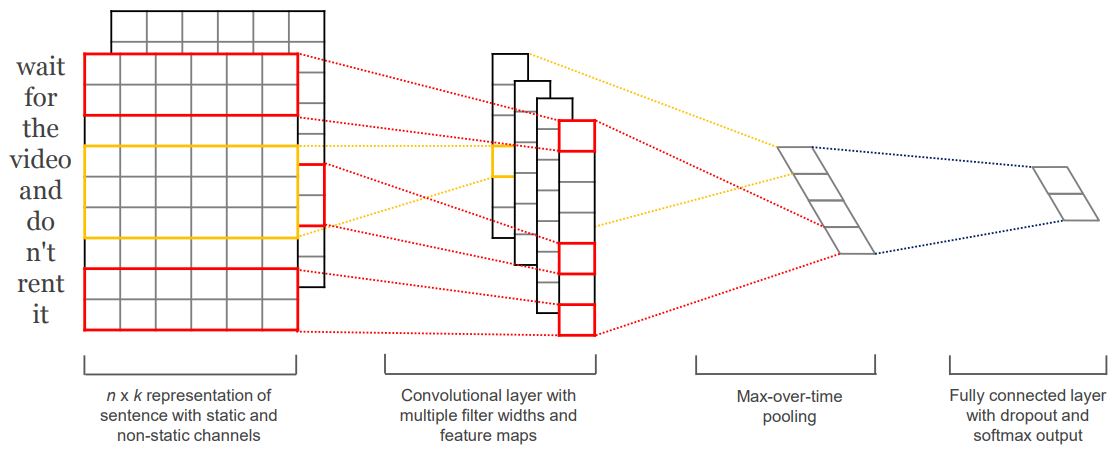
\includegraphics[width=\textwidth]{images/cnn_text.png}
    \caption{CNN for sentence classification}
    \label{fig:cnn}
\end{figure}

CNNs are capable of computing vectors for all possible sub-phrases in a sentence, not just grammatically correct one as done by RNNs. A CNN takes an input sentence of word length $n$ where each word is represented distributively in $d$ dimension. So the input $X_{1:n}$ is a $2D$ matrix of shape $n \times d$  where $x_{i}$ $\epsilon$ $\mathbb{R}^d$. Input $X_{1:n}$ can be represented as \cref{eq:cnn_input}.

\begin{equation}
    \label{eq:cnn_input}
    X_{1:n} = x_{1} \oplus x_{2} \oplus \cdots \oplus x_{n}
\end{equation}

where $\oplus$ is the concatenation operator. On the input layer, convolution filter $W$  $\epsilon$ $\mathbb{R}^{hd}$ is applied over window of $h$ words to generate a new feature. So, a feature $c_{i}$ is generated from the word window $x_{i:i+h-1}$ with the following operation:

\begin{equation}
    c_{i} = \sigma (Wx_{i:i+h-1} + b)
\end{equation}

where $W$ is the weight matrix for the connections, $\sigma$ is the activation function and $b$ $\epsilon$ $\mathbb{R}$ is the bias. Now, this filter is applied to each possible window of words giving an feature map $C$ $\epsilon$ $\mathbb{R}^{n-h+1}$.

\begin{equation}
    C = [c_{1}, c_{2}, \cdots, c_{n-h+1}]
\end{equation}

The entries in feature map $C$ are sharing the parameter $W$, where each $c_{i}$ $\epsilon$ $C$ is a result of calculation on small segment of the input. Then a $max-pooling$ operation is applied on these feature maps to capture the most important part.

\begin{equation}
    \Tilde{C} = max(C)
\end{equation}

This parameter sharing helps the model to incorporate an inductive bias into the model, helping to become learn the location invariant local features. There are $k$ number of filters applied to the input with different window sizes which are then concatenated to form a vector $\textbf{K}$ $\epsilon$ $\mathbb{R}^k$. Which is then fed to next hidden layer or output layer.

An illustrated diagram of an CNN architecture for text classification is shown in fig \cref{fig:cnn} \footnote{taken from \cite{kim2014convolutional}}.

\subsubsection{Sequence  to Sequence Models}
Most of the NLP tasks require sequential output instead of a single output label unlike classification or regression \cite{sutskever2014sequence}. These tasks can be Machine Translation of natural language, Question-Answering or Summary generation systems. These systems take a sequence of input and process it to produce yet another sequence for output. The goal is to take a sequence $(x_{1}, x_{2}, \cdots, x_{n})$ as input and map it to another sequence $(y_{1}, y_{2}, \cdots, y_{n})$ as output.

The architecture used to deal with these kind of problems is known as Sequence to Sequence model or in common terms, seq2seq model. It is a combination of auto-encoders and decoders which works in a sequential manner where encoder is an neural architecture to generate a context vector from input sequence and decoder, another neural architecture taking context vector as input and generating the output sequence.

The encoder takes an input $X$ and maps it to fixed size context vector $Z$ using the formula \cref{eq:enc}

\begin{equation}
    \label{eq:enc}
        Z = \sigma(WX + b)
\end{equation}

where $\sigma$ is activation function. A decoder then maps the context vector $Z$ to a new form of input $X^{\prime}$ as shown in equation \cref{eq:dec}

\begin{equation}
    \label{eq:dec}
        X^{\prime} = \sigma^{\prime}(W^{\prime}Z + b^{\prime})
\end{equation}

where $\sigma^{\prime}$ is another activation function. The loss is calculated as the squared error between original and reconstructed input as shown in equation \cref{eq:seq2seq_loss}. An illustrated diagram of seq2seq model is shown in fig \cref{fig:enc_dec} \footnote{Taken from \url{http://web.stanford.edu/class/cs224n/}}.

\begin{equation}
    \label{eq:seq2seq_loss}
        L = ||X-X^{\prime}||^{2}
\end{equation}

\begin{figure}
     \centering
     \begin{subfigure}[b]{0.25\textwidth}
         \centering
         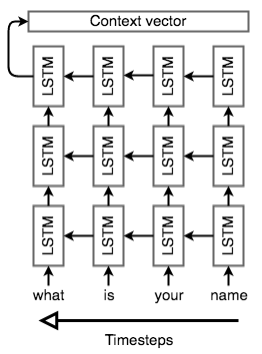
\includegraphics[width=\textwidth]{images/encoder.png}
         \caption{Encoder}
         \label{fig:encoder}
     \end{subfigure}
    %  \hfill
     \begin{subfigure}[b]{0.25\textwidth}
         \centering
         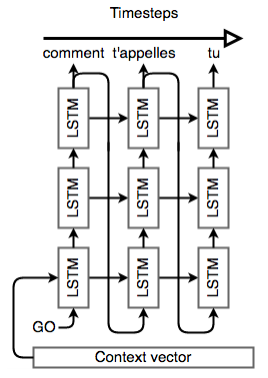
\includegraphics[width=\textwidth]{images/decoder.png}
         \caption{Decoder}
         \label{fig:decoder}
     \end{subfigure}
        \caption{Encoder-Decoder architecture using LSTM for seq2seq model}
        \label{fig:enc_dec}
\end{figure}

\paragraph{Attention} A problem with general encoder-decoder model is that they give equal importance to all the parts of input sequence. Also, the input sequence is compressed into a single context vector which creates the bottleneck problem, where a long information is tried to be kept into one small representation. 

A solution to this problem was proposed in the work \cite{bahdanau2014neural} introducing a new mechanism called Attention. Attention aligns the output at each decoding step to the whole input sequence in order to learn the most important part of the input aligning with the current step output by providing an attentive output.

Let's say we have calculated the encoding hidden states $(h_{1},  h_{2}, \cdots, h_{n})$ for the input sequence $(x_{1}, x_{2}, \cdots, x_{n})$ during the calculation of context vector $Z$. For a decoder hidden state $s_{t}$ on timestep $t$, we get attention score $e^{t}$ as follows:

\begin{equation}
    \label{eq:att_score}
        e^{t} = [s^{T}_{t}h_{1}, \cdots, s^{T}_{t}h_{n}]
\end{equation}

We take the softmax of these scores to get the attention distribution at timestep $t$.

\begin{equation}
    \label{eq:att_dist}
        \alpha^{t} = softmax(e^{t})
\end{equation}

The attention output $a_{t}$ is then calculated as the weighted sum of encoder hidden state using $\alpha^{t}$:

\begin{equation}
    \label{eq:att_out}
        a_{t} = \sum_{i=1}^{n} \alpha_{i}^{t}h_{i}
\end{equation}

Finally, we concatenate the attention output $a_{t}$ with decoder hidden state $s_{t}$ and proceed to calculate the negative log loss same as the non-attention decoder model.

\subsubsection{Contextual Word Embeddings}\label{sec:context_we}
As discussed in \cref{sec:word_emb}, the word embeddings generated by algorithms like word2vec \cite{mikolov2013distributed} and GloVe \cite{pennington2014glove} lacks the contextual awareness and fail to differentiate a word with different sense. For example, word $get$ has thirty different senses (meaning) in wordnet \footnote{\url{https://wordnet.princeton.edu/}} based on the different contexts. But if we use pre-trained word embeddings to generate the vector representation of $get$, it will be same for all the thirty times and we will loose the semantic information. 

A new trend of transfer learning came in Deep Learning based NLP with the introduction works like ELMo \cite{peters2018deep} and ULMFiT \cite{howard2018universal} where language models are used to learn the nuances of the language grammar and then the pre-trained language model is then fine-tuned on a task specific dataset to achieve better results.

\begin{figure}
    \centering
    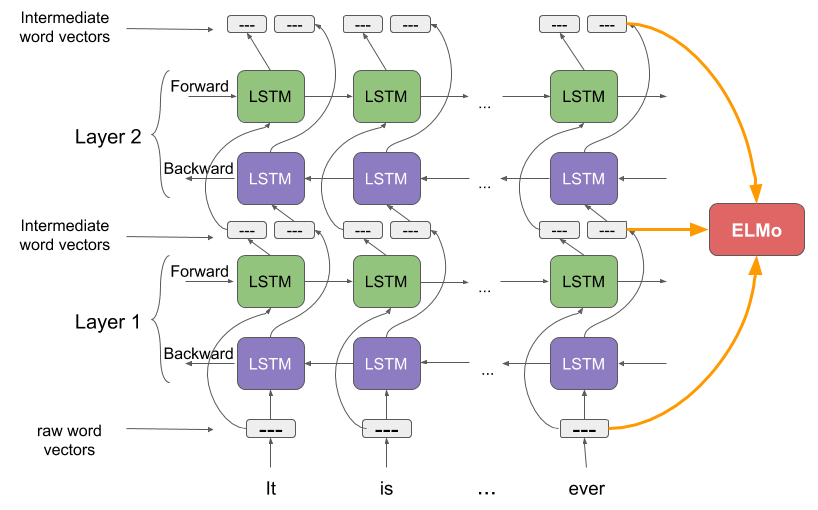
\includegraphics[width=0.75\textwidth]{images/elmo.png}
    \caption{ELMo Vector Representation}
    \label{fig:elmo}
\end{figure}

\paragraph{ELMo} stands for Embeddings Learned from Language Models \cite{peters2018deep} uses a bidirectional language model to capture the context of a word in a sentence from both sides (left to right and vice-versa). ELMo uses an character-level CNN to convert raw text into a word vector which is then fed into a bidirectional language model. The ouput of this BiLM is then sent to the next layer of BiLM to form a set of intermediate word vectors. The final output of ELMo is the weighted sum of raw vectors and the intermediate vectors formed from two layers of the BiLMs. The two language models used here are based on LSTM architectures. An illustration of ELMo is shown is \cref{fig:elmo} \footnote{Taken from \url{https://www.analyticsvidhya.com/blog/2019/03/learn-to-use-elmo-to-extract-features-from-text/}}.

ELMo achieved 9\% error reduction on the SQuAD (question-answering) dataset compared to then state-of-the-art, 16\% on Ontonotes SRL dataset, 10\% on Ontonotes coreference dataset and 4\% on CoNLL 2003 dataset. It paved a huge path in the success of contextualized word representations for different tasks in NLP.

\paragraph{ULMFiT} stands for Universal Language Model Fine Tuning, introduced the way of applying transfer learning on text classification problem \cite{howard2018universal}. It does so in three main steps: first, train an general domain language model on large corpus of text (mainly Wikipedia); second, fine tune the language model on task specific target dataset; and third, use the again fine tune the fine-tuned language model as classifier by adding a softmax activation on top with target dataset. An illustration of the three steps of ULMFiT is shown in \cref{fig:ulmfit_steps}.

% \begin{figure}
%     \centering
%     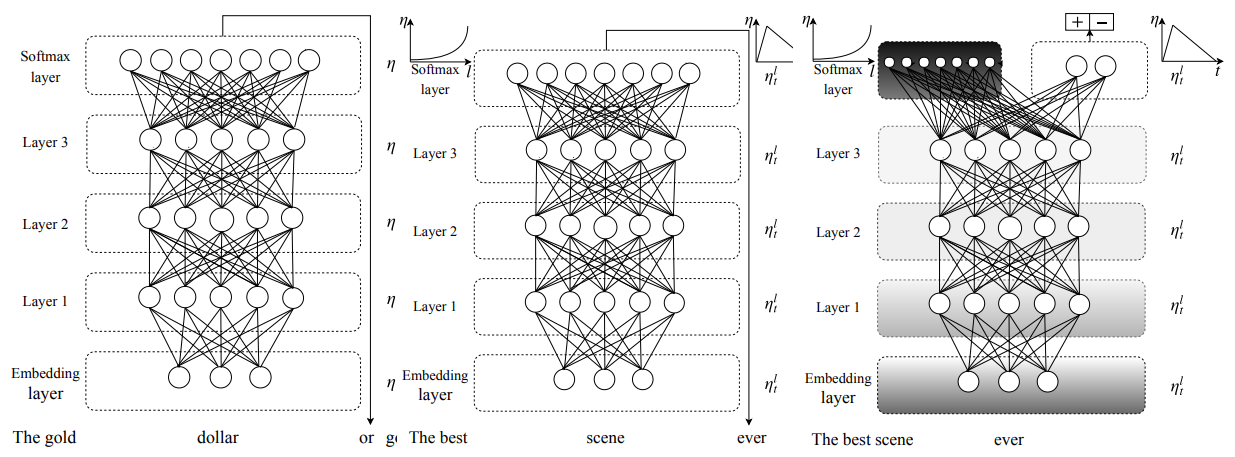
\includegraphics[width=\textwidth]{images/ulmfit.png}
%     \caption{ULMFiT Steps}
%     \label{fig:ulmfit}
% \end{figure}

\begin{figure}
     \centering
     \begin{subfigure}[b]{0.3\textwidth}
         \centering
         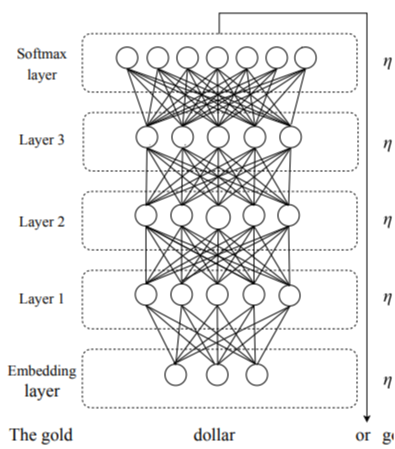
\includegraphics[width=\textwidth]{images/ulm1.png}
         \caption{LM Training}
         \label{fig:lm_train}
     \end{subfigure}
    %  \hfill
     \begin{subfigure}[b]{0.3\textwidth}
         \centering
         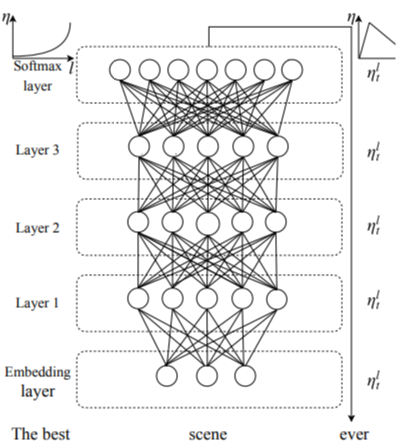
\includegraphics[width=\textwidth]{images/ulm2.png}
         \caption{LM Fine-Tuning}
         \label{fig:lm_ft}
     \end{subfigure}
    %  \hfill
     \begin{subfigure}[b]{0.3\textwidth}
         \centering
         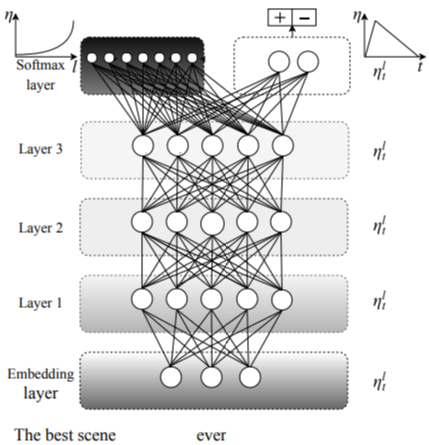
\includegraphics[width=\textwidth]{images/ulm3.png}
         \caption{Classifier Training}
         \label{fig:lm_classif}
     \end{subfigure}
        \caption{ULMFiT Steps \cite{howard2018universal}}
        \label{fig:ulmfit_steps}
\end{figure}


ULMFiT achieved better results for text classification on six different datasets ranging from topic classification to sentiment analysis. It did so by learning the general rules of grammar from huge corpus of text and then transferring that learning with fine tuning on a task-specific dataset providing better results than state-of-the-arts \cite{howard2018universal}.

\subsubsection{Transformers}\label{sec:transformers}
Almost all of the models we discussed have recurrent behaviour, which can not be trained parallely. This imposes a huge problem of time taken to train a model from scratch. In the work \cite{vaswani2017attention}, authors proposed a new neural architecture called Transformers which uses a combination of self attention and feed-forward network in its encoder-decoder model and doesn't require any recurrent or convolutional elements. This new seq2seq model was a huge success where it gained better performance on various sequential NLP tasks. To name one, it improved the machine translation performance by 10\% on WMT EN-FR and WMT EN-DE datasets. It also reduced the training time by large margin benefiting its non-recurrent nature \cite{vaswani2017attention}.

The success of transformer architecture paved the way for development of new models to solve the sequential tasks. It helped NLP researchers to utilize its non-recurrent nature in transfer learning where the transformer is used for general pre-training of a language model on large corpus of text which can be used for fine-tuning on domain specific dataset for downstream tasks. An encoder-decoder model of Transformer architecture is shown in the \cref{fig:trans}.

\begin{figure}
    \centering
    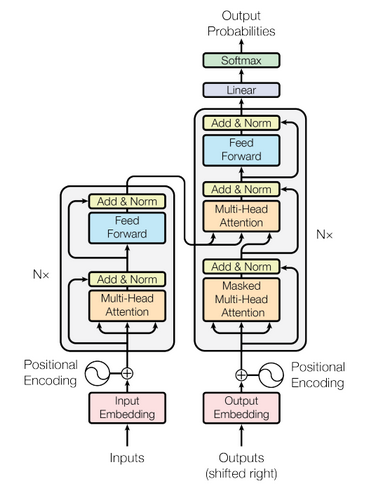
\includegraphics[width=0.5\textwidth]{images/transformer.png}
    \caption{Transformer architecture \cite{vaswani2017attention}.}
    \label{fig:trans}
\end{figure}

\paragraph{Generative Pre-Training}
One of the earliest works in using Transformers for pre-training of language model was presented in \cite{radford2018improving}. Following the idea from ELMo \cite{peters2018deep}, authors proposed a language model using transformer decoder trained on large corpus and then fine-tuned on task specific dataset. The main difference of GPT from ELMo is that ELMo uses two independent LSTM language models to caputre the forwards and backward context whereas in case of GPT, it uses a uni-directional multi-layer transformer language model capable of capturing context due to its attentive nature.

ELMo takes a feature based approach of feeding feature vectors for different tasks into different models, whereas GPT takes a fine-tuning based approach where same language model trained on huge corpus is fine-tuned for downstream tasks without changing the architecture. An illustration of a GPT model used for pre-training is shown in \cref{fig:gpt} \footnote{Taken from \url{https://openai.com/blog/language-unsupervised/}}.

\begin{figure}
    \centering
    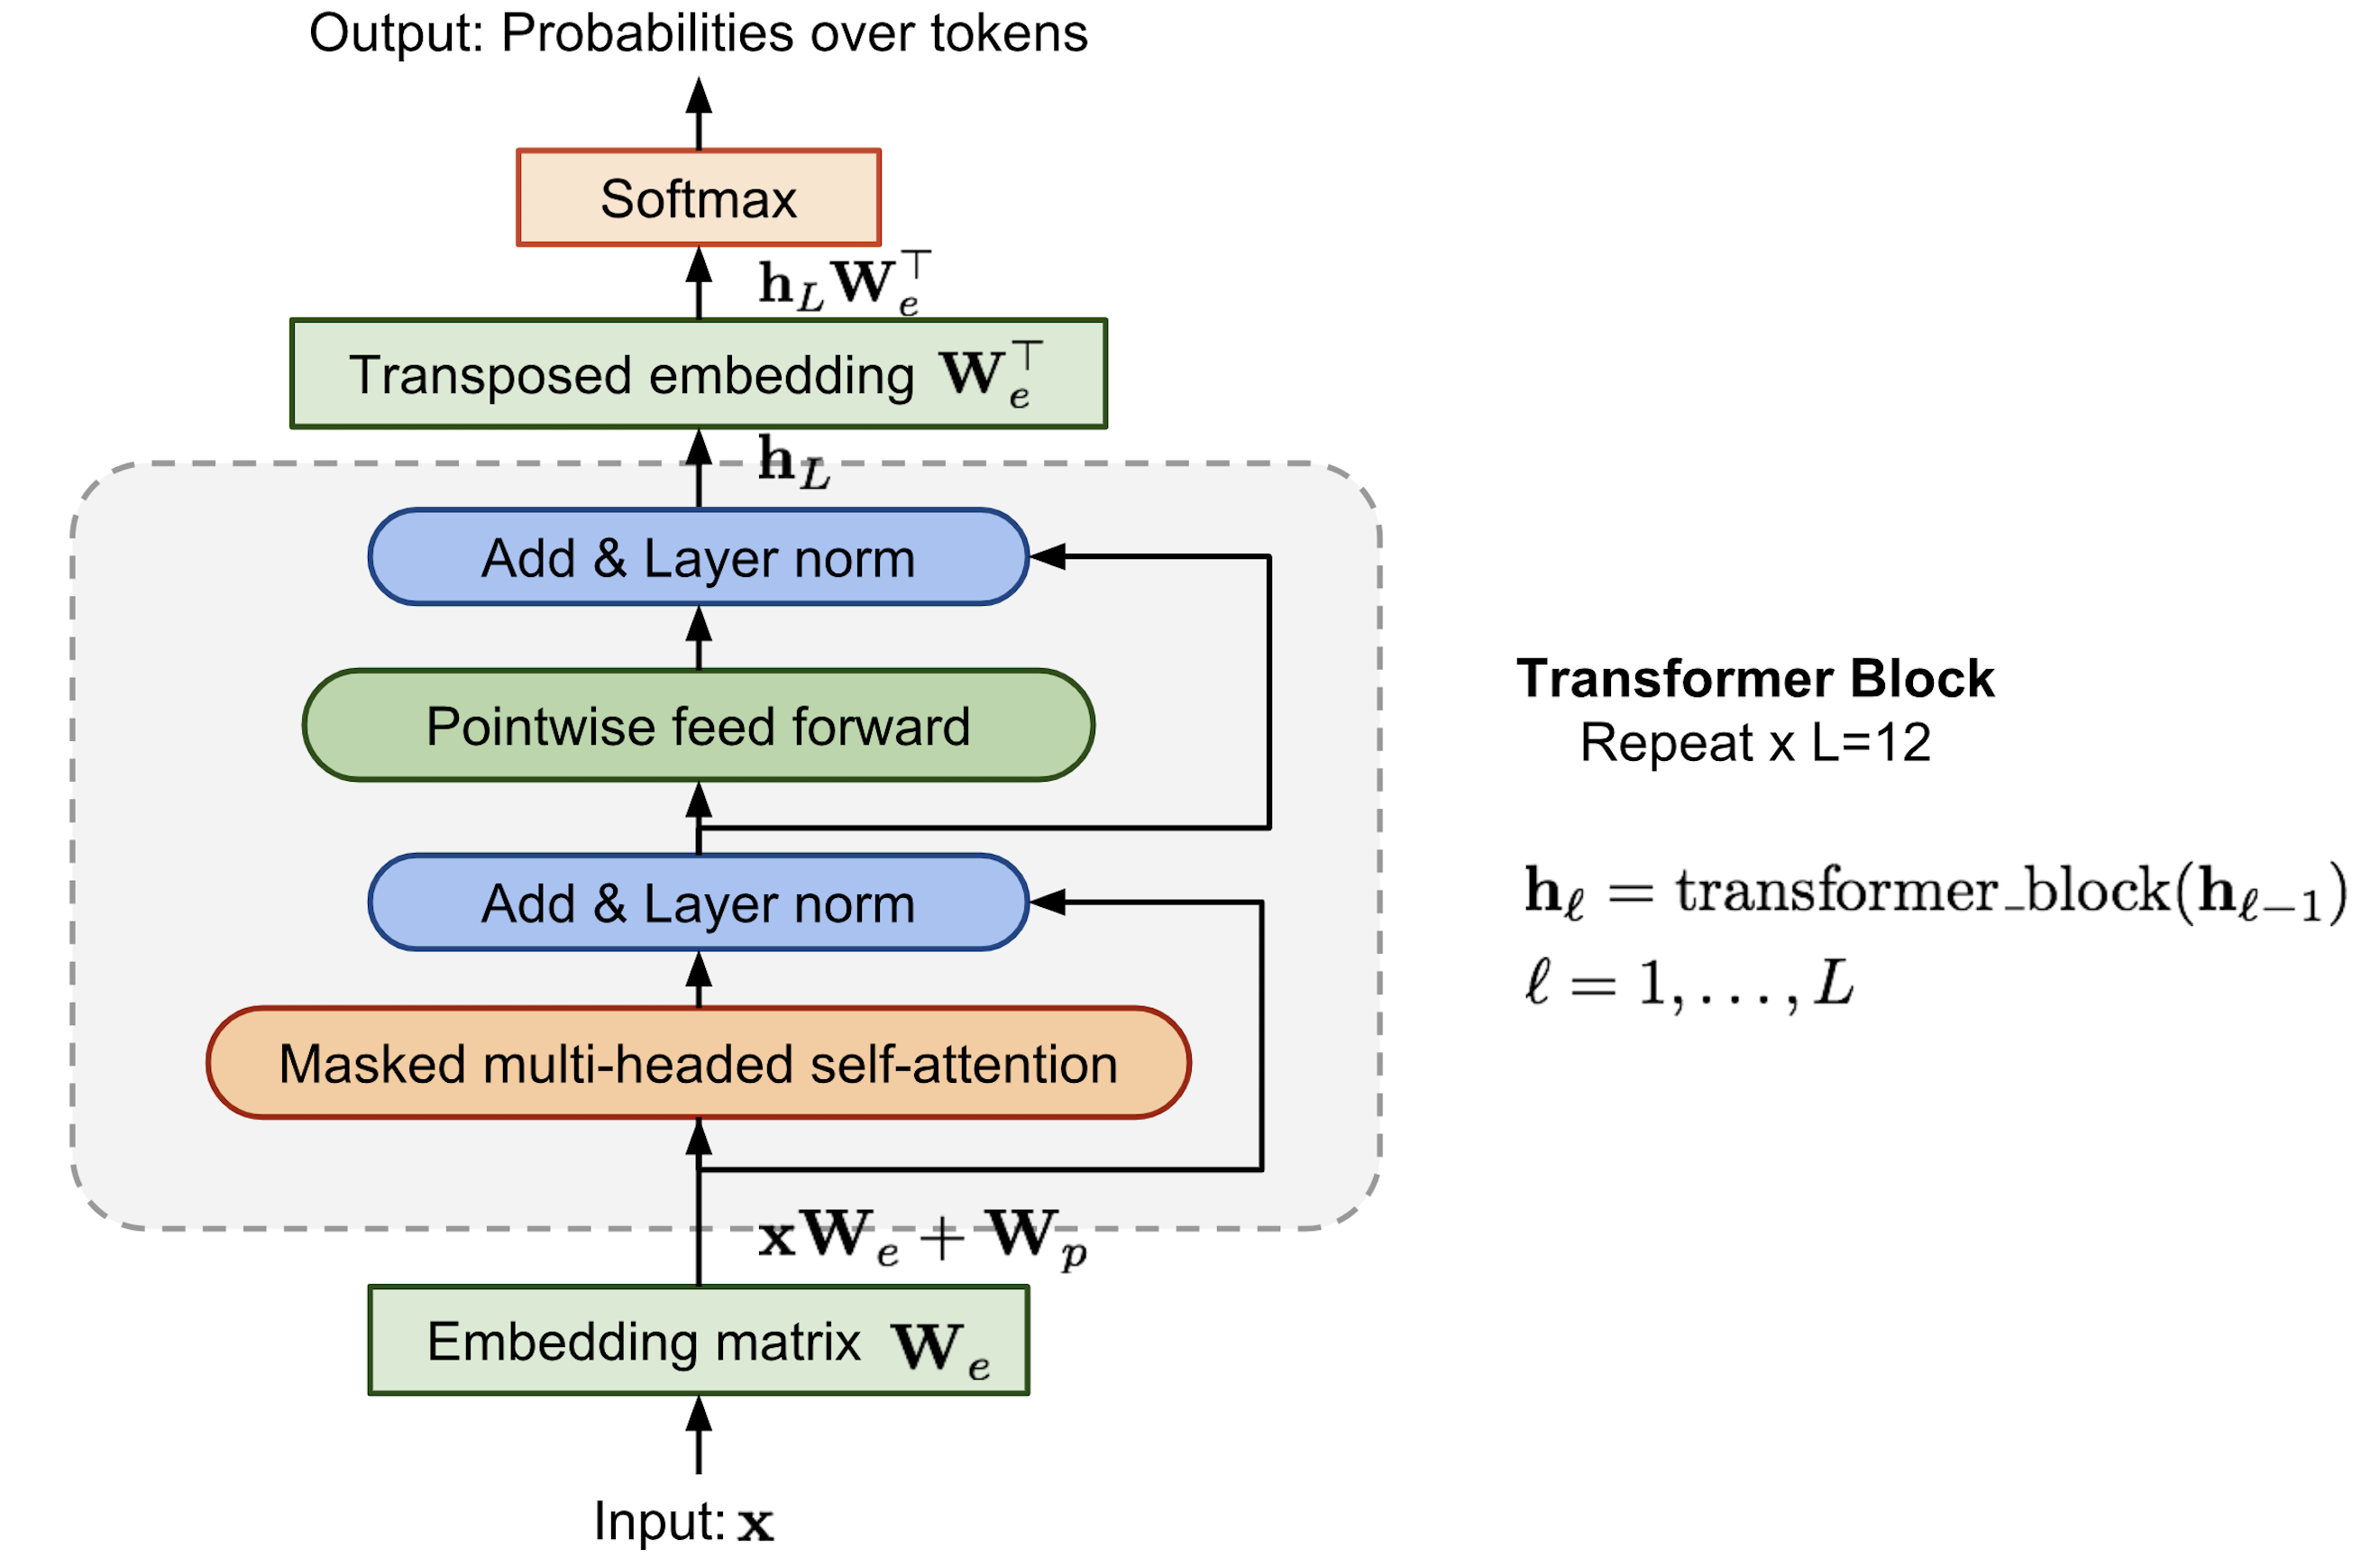
\includegraphics[width=0.75\textwidth]{images/GPT.png}
    \caption{GPT architecture.}
    \label{fig:gpt}
\end{figure}

\paragraph{Bidirectional Encoder Representation from Transformers}
BERT \cite{devlin2018bert} is another example of the success of transfer learning in NLP. BERT is a bidirectional transformer language model trained on a large text corpus that can be fine-tuned on any domain specific dataset for the downstream tasks like text classification or named entity recognition. BERT mainly differs from other models like GPT and ELMo because of the pre-training tasks used during the unsupervised training of language model. It involves two tasks; first, Masked Language Model (MLM) \cite{taylor1953cloze} or prediction of the masked word in a sentence, and second, prediction of next sentence from the corpora.

For the first task of Masked Language Model, let’s say we have a sentence ‘Boris Johnson is the Prime Minister of UK’. So instead of training for prediction of next word in the sentence as a general Language Model, BERT pre-training replaces 15\% of the words with a [MASK] token and learns to predict the correct word at the position of [MASK] token. In the second task of Next Sentence Prediction, the model is trained to learn the relationship between sentences where for a given sentence pair A \& B, the model is asked to predict if the sentence B is actually the next sentence that comes after A or not?

BERT improved the fine-tuning based approach of GPT by using a bidirectional transformer for masked language modelling by learning the both left and right context which is a huge improved over GPT's unidirectional approach specially for token-level tasks like Question Answering where the answer depends on both left and right contexts. An illustrated diagram of BERT pre-training and fine-tuning is shown in \cref{fig:bert1}. 
% A visual comparison between BERT, GPT and ELMo architectures presented in the work \cite{devlin2018bert} is shown in \cref{fig:bert2}.

\begin{figure}
    \centering
    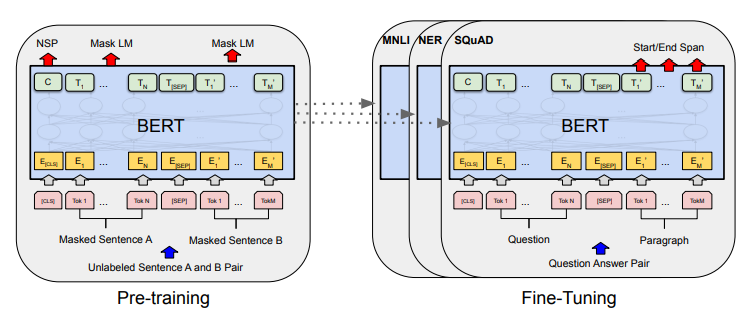
\includegraphics[width=0.75\textwidth]{images/bert1.png}
    \caption{BERT \cite{devlin2018bert}}
    \label{fig:bert1}
\end{figure}


% \begin{figure}
%     \centering
%     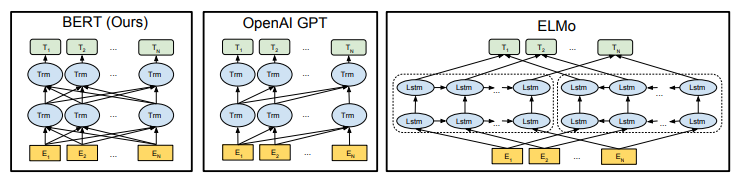
\includegraphics[width=\textwidth]{images/bert2.png}
%     \caption{BERT, GPT and ELMo \cite{devlin2018bert}}
%     \label{fig:bert2}
% \end{figure}


% \subsection{Current State-of-the-Art}\label{sec:sotas}
In the literature, current State-of-the-Arts (SOTA) for almost all of the NLP tasks are based on deep learning learning algorithms. In the \cref{tab:sotas} we will list few works and their performance on the tasks defined in \cref{sec:tasks}.

\begin{sidewaystable}[!htbp]
  \begin{center}
    \caption{Current State-of-the-Arts. We can see that almost all of the works are based on deep learning.}
    \label{tab:sotas}
    \begin{tabular}{|c|c|c|c|c|}
      \hline
      \textbf{Task} & \textbf{Work} & \textbf{Model} & \textbf{Performance} & \textbf{Data}\\
      \hline
      \textbf{NER} & \cite{baevski2019cloze} & CNN Large + fine-tune & 93.5 F1 & CoNLL 2003\\
      & \cite{strakova-etal-2019-neural} & LSTM-CRF+ELMo+BERT+Flair & 93.38 F1 & CoNLL 2003\\
      \hline
      \textbf{POS Tagging} & \cite{Bohnet_2018} & Meta BiLSTM & 97.96 Acc & Penn Treebank\\
      & \cite{Heinzerling_2019} & Multilingual BERT and BPEmb & 96.77 Acc &  Universal Dependencies\\
      \hline
      \textbf{NLI} & \cite{liu2019roberta} & RoBERTa & 90.8 Acc & Multi-NLI\\
      & \cite{yang2019xlnet} & XLNet-Large & 90.2 Acc & Multi-NLI\\
      \hline
      \textbf{Relation Extraction} & \cite{lai-etal-2018-sunnynlp} & SVM with GloVe & 0.76 F1 & SemEval 2018 Task 10\\
      & \cite{baldini-soares-etal-2019-matching} & BERT: Matching-the-Blanks & 89.5 F1 & SemEval 2010 Task 8\\
    %   \hline
    %   SRL & \cite{he-etal-2018-jointly} & ELMo Modified & 85.5 & OntoNotes\\
    %   & \cite{peters2018deep} & ELMo & 84.6 & OntoNotes\\
    %   \hline
    %   Dependency Parsing & 25.113231 & d &   & Penn Treebank\\
    %   & 1110.1 & a &   & Universal Dependencies\\
      \hline
      \textbf{Machine Translation} & \cite{edunov2018understanding} & Transformer Big & 35 BLEU  & WMT 2014 EN-DE\\
      & \cite{edunov2018understanding} & Transformer Big & 45.6 & WMT 2014 EN-FR\\
    %   \hline
    %   Data Augmentation & 25.113231 & d &   & imdb\\
    %   & 1110.1 & a &   & Amazon Reviews\\
    %   \hline
    %   Summary Generation & 25.113231 & d &   & CNN/Daily Mail\\
    %   & 1110.1 & a &   & CNN/Daily Mail\\
      \hline
      \textbf{Question Answering} & \cite{lan2019albert} & ALBERT (ensemble model) & 92.21 F1 & SQuAD\\
      & \cite{lan2019albert} & ALBERT (single model) & 90.9 F1 & SQuAD\\
      \hline
      \textbf{Text Classification} & \cite{yang2019xlnet} & XLNet & 0.62 Error & Dbpedia\\ 
      & \cite{yang2019xlnet} & XLNet & 4.49 Error & AG News\\
    %   \hline
    %   Aspect-Based Sentiment & 25.113231 & d &   & SemEval-2014 Task 4\\
    %   & 1110.1 & a &   & SemEval-2014 Task 4\\
      \hline
    \end{tabular}
  \end{center}
\end{sidewaystable}

% \subsection{Business Process}\label{business_process}
% % \label{sec:use_in_business}
% \paragraph{Cold Start \& Concept Drift} We have seen from the \cref{tab:sotas} that deep learning has given better results with ample amount of data available for training. But the problem in a business process is with the availability of data itself. Deep learning can provide better performance but will require a huge amount of resource to train the models. 

% In a business process it is hard to get ample amount of data in the initial phase and hence we face the problem of cold start. We need to train our models with less data only, which results in reduced performance. Also, in a business process we keep receiving data as time goes on like stream of data. After some times, we may get new data that might be enough to train a deep learning model. And there is high chance that the relationship between problem and solution changes as well. Hence it is important to address the problem of concept drift as well.

% Less Data

% Class Imbalance

% But deep learning has its own consequences, and that is the resource needed for the training of a deep learning model. It takes a lot of labelled data for training a deep learning model, as well as the training itself takes a long time and very powerful system to run the process on. Even if we can out-source the training process to cloud services like AWS or Azure, we may reduce our expenses on time and machine but still we will need a lot of training data that should be labelled.

% These can be solved with methods like One shot learning or data augmentation to increase the training set. GANs

% With a general semi-supervised training on big corpus, the learning can be transferred to some domain specific task with minimal fine tuning for particular task.

% \subsection{Concept Drift}
% In industry, collecting a training data brings a new form of challenge: the challenge of concept drift. The problem is that during the start of a business process 

% \clearpage

\section{Proposed Methodology}\label{sec:methods}
In order to achieve our objectives we hope to adopt the following methodologies.

\subsection[Objective 1]{Objective 1}
\textit{``Identifying the NLP related problems in business processes that are not well addressed by academic research''}

\vspace{12pt}
\noindent Academic research can overly simplify a real-world problem in order to gain good performance. For example, the data used may have training samples which are different to those in real world business process. In real scenarios, getting enough labelled data is usually a problem as the data generation is also a part of the process. We might get very less data during the start of the process or even if the data is available that will be unlabelled. The quality of the data may be poor, and we need to apply pre-processing before we can use that data for any experiment. We will identify these kind of problems which arise during the implementation of machine learning methods in real-world application. 

We plan to investigate two approaches for identifying these problems faced by business processes. First, by investigation of literature where we will do extensive review of current state-of-the-art methods from academic research and try to find out where they can fail while implementing them in real-world scenario. Second, by talking to the representatives of different industries to establish at first hand where the key challenges lie in adopting the state-of-the-art methods from academic research in their tasks.

\paragraph{Deliverable:} At the end of this phase, we will disseminate our findings in form of review paper or report through journal publications.

\subsection{Objective 2}
\textit{``Identifying the common use-cases from business processes and gathering data for those use-cases''}

\vspace{12pt}
\noindent There are various use-cases in business process like text classification, natural language generation or question answering. We will identify some use-cases that are very common in business processes in terms of text mining throughout the industry. This will again be achieved by either contemplation or by talking to people from industry.

While selecting the use-case, focus will also be on the availability of public datasets that can be used to easily simulate the real-world scenario. We will try to ask some companies if they are willing to share their data in exchange to better methods for their business process.

\paragraph{Deliverable:} At the end of this phase, any dataset gathered will be made available to the community through open repositories like UCI ML Repo \footnote{\url{https://archive.ics.uci.edu/ml/index.php}}.

\subsection{Objective 3}
\textit{``Setting up the benchmark performance by implementing state-of-the-art algorithms for the real-world scenario''}

\vspace{12pt}

\noindent We will use public datasets to simulate the real-world scenario and apply the current state-of-the-art. For example, adding timestamps to a pre-processed public datasets can help in simulating a real-world scenario. Then with time-stamps we can simulate the cold-start scenario where initially we will have very less data to start our process and then the labelled data will be generated as a part of the process. 

We will use this real-world scenario to test the various state-of-the-art methods from literature review on the use-cases selected from objective 2. 

\paragraph{Deliverable:} At the end of this phase, we will publish our findings in form of through various workshops and conferences focused on solving NLP related problems in business processes.

\subsection{Objective 4}
\textit{``Developing novel methods to outperform the current state-of-the-art algorithms and evaluating them with real world data on different use-cases''}

\vspace{12pt}

One of the possible problems can be the unavailability of labelled data for training the learning models. To gain better performance with less training data, we can either develop techniques suitable for working with less training data; or develop techniques for generating the new training data.

\subsubsection{Reducing the Data Requirement}
We can take an approach to develop novel techniques that can give good performance on less data. Chunking the time period based on the availability of labelled data can be one way, where we will use different set of algorithms for based on the amount of labelled data available for training.

In the initial phase, where we have very less amount of labelled data for training we can use rule-based traditional NLP techniques. After some time, when we develop more labelled data we can use feature engineering based machine learning techniques for better performance. After a long time, when we have a huge corpus of labelled data for training then we can deep learning techniques suitable for that amount of training data. A similar kind of initial work is explained in \cref{sec:wetc}.

\subsubsection{Generating New Training Data}
Another way can be augmenting data to increase the amount of training data. Data augmentation in NLP is still not very popular as compared to that in Computer Vision \cite{guo2018long}. The few techniques used in NLP for augmenting text data from literature that can be adopted and extended are;

\paragraph{Back Translation} 
In this method, a sentence is translated from one language to other and then again back translated to the first language. In this process of back translation, some of the words are changed from the original sentence while maintaining the semantics as it is. Similar kind of work is done here \cite{Xie2019} for consistency training.

\paragraph{Contextual Word Replacement}
Another good technique for augmentation is randomly replacing some of the words with their synonyms/antonyms with changing the context of the whole sentence. This technique was introduced in the work \cite{kobayashi2018contextual} which achieved comparatively better results on various datasets.

\paragraph{GANs}
Generative Adversarial Networks are very successful in computer vision for new data generation \cite{ali2019mfc}. But they are not much investigated in text for the same purpose  \cite{guo2018long}. There are few examples like MaskGAN and LeakGAN \cite{fedus2018maskgan,guo2018long} which can be tested and improved for our purpose.

\vspace{6pt}
\paragraph{Deliverable:} At the end of this phase, we will disseminate our findings through different conferences and journals in form of technical papers and will also make our code open-source through GitHub \footnote{\url{https://github.com/}} or some other open-source code sharing platforms.

% might not be available for training the learning algorithms.

% \subsection{Objective 1}
% Transfer learning has gained a lot of success in the Computer Vision based deep learning tasks. The weights trained on a huge corpus like Imagenet are shared for smaller tasks that increase the performance after fine-tuning. The models trained on huge corpus are able to identify the general features of an image and after fine-tuning the models they pass their learning to smaller domain specific tasks. 

% In the last couple of years, transfer learning has also gained popularity in NLP research. The idea here is to train a Language Model on a huge general corpus like Wikipedia text or news corpus which will help model in learning the basics of grammar and understanding its rule. Then fine-tune the language model on a domain specific corpus according to the need. The models discussed in literature like ULMFiT and BERT are based on this idea only. 

% These works have shown very good performance on the pre-processed public datasets. But there is not much evidence of their performance on the real world data, where either data is available in very less amount or is available in streams. As shown in \cref{sec:initial_work}, deep learning has potential to enhance NLP performance in business process provided the problem of data availability is tackled.

% By comparing traditional NLP techniques with these machine/deep learning techniques on various scenarios, we will identify the gaps between industry and academia. By modifying public datasets with time-stamp marks we can simulate a business process environment with cold start and concept drift scenario. We will propose new algorithms based on transfer learning in NLP to bridge the gap between industrial solutions and academic research. 
% % In the initial phase, the NLP solutions based on feature engineering will be applied on the some custom or public datastes and then these methods will be compared with our new proposed deep learning  based methods. 

% \subsection{Objective 2}
% Training deep learning models requires a huge amount of labelled data and in a business process we often face the problem of cold start where its not always easy to get the ample amount of labelled data in the initial phase. To tackle this problem, we can take two approach; first, develop techniques suitable for giving good performance on less training data; or second, develop techniques for increasing training data.

% \subsubsection{Reducing the Data Requirement}
% We can take an approach to develop novel techniques that can give good performance on less data. Chunking the time period based on the availability of labelled data can be one way, where we will use different set of algorithms for based on the amount of labelled data available for training.

% In the initial phase, where we have very less amount of labelled data for training we can use rule-based traditional NLP techniques. After some time, when we develop more labelled data we can use feature engineering based machine learning techniques for better performance. After a long time, when we have a huge corpus of labelled data for training then we can deep learning techniques suitable for that amount of training data. A similar kind of initial work is explained in \cref{sec:wetc}.


% \subsubsection{Augmenting Training Data}
% Another way can be making use of data augmentation to increase the amount of training data. Data augmentation in NLP is still not very popular as compared to that in Computer Vision. The few techniques used in NLP for augmenting text data from literature that can be adopted and extended are;

% \paragraph{Back Translation} 
% In this method, a sentence is translated from one language to other and then again back translated to the first language. In this process of back translation, some of the words are changed from the original sentence while maintaining the semantics as it is. Similar kind of work is done here \cite{Xie2019} for consistency training.

% \paragraph{Contextual Word Replacement}
% Another good technique for augmentation is randomly replacing some of the words with their synonyms/antonyms with changing the context of the whole sentence. This technique was introduced in the work \cite{kobayashi2018contextual} which achieved comparatively better results on various datasets.

% \paragraph{GANs}
% Generative Adversarial Networks are quite popular in CV for new data generation. But they are not much investigated in text for the same purpose. There are few examples LeakGAN like which can be tested and improved for our purpose \cite{guo2018long}.

% % \subsection{Objective 3}
% % After sometimes, when new labelled data is available, why not to use it and identify any drift of concept rather than using a system trained on synthetic data.
% % % Handling Concept Drift

% \subsection{Evaluation}\label{sec:eval}
% We will evaluate our proposed methods with various real life use-cases

% \subsection{Dissemination}
% Any type of dataset created by us will be made publicly available through UCI Machine Learning repository \footnote{\url{https://archive.ics.uci.edu/ml/index.php}}. At each stage of the research we will make our finding public through conferences and journal publications. The code will be made publicly available through GitHub \footnote{\url{https://github.com/}}.



% Develop machine and deep learning algorithms to support the NLP rules. However, learning algorithms need large amounts of data for training to produce good results. But getting good labelled data is expensive. There is a trade-off between performance and data availability. Prof. Andrew Ng of Stanford University identifies that “we need to focus on developing better algorithms that can work on smaller datasets and stop relying on a large amount of data to train the models”. In our case also, we need to develop representation and methods that can work on small amount of data provided for training. For this, methods like One-Shot Learning or Siamese Networks can be explored to train the models on smaller datasets [5]. Furthermore, evolutionary algorithms can be used to develop an approach of selecting best possible representation and method from a set of different representations and methods for training the machine learning/deep learning models [6].

% In the final step, we need to use the boosting mechanisms that employ feedback to learn from our system errors in order to improve the performance. In traditional machine learning there are well-established boosting techniques available that can be used to fulfil the purpose, whereas in deep learning tree methods like gcForest can be explored a potential approaches to developing effective boosting mechanism.

% \clearpage

\section{Initial Work}\label{sec:initial_work}
We have done some initial work for addressing text mining problems in business process in two use cases:

\subsection{Natural Language Generation (NLG)}

\subsubsection{Obituary Generation}
In the ongoing Interface funded project of Obituary generation at CSDM school, we are working to generate the obituary of a deceased person based on the details given about the person. We have collected the data of obituaries from one of the most famous obituary website of UK named Funeral Notices \footnote{\url{http://funeral-notices.co.uk/}}. We have selected notices only from the Scotland area and those posted after 2015. 

In the initial phase we are taking a Case-Based approach where the problem set is represented with the various features related to deceased person's life, family and funeral details. One of the commencing tasks for this approach is to develop a labelled dataset with all the features marked in the funeral notices. 
% This approach can also be termed as template filling approach.

The work is currently in progress and after the CBR implementation, we are going to take a Natural Language Generation (NLG) approach using deep learning to generate the new text based on the features given as the input to the model. 
% We will be using the transformers trained on huge datasets with millions of hyper-parameters by fine-tuning them on our custom dataset.

\subsection{Text Classification}

\subsubsection{Compliance Management}
In the recent OGIC funded AZOTH project at CSDM school, we worked on the knowledge extraction and requirement mapping on Oil and Gas regulatory documents. One of the problem statement was to identify if an extracted sentence from a document is a Compliance Requirement (CR) or not? The dataset consists of 2,600 sentences which have been determined as: 

\begin{enumerate}
    \item accept (known CR);
    \item postpone (possible CR but requires further review); and 
    \item reject (known non-CR); with respect to their CR status. 
\end{enumerate}

As a result, this is considered a classification problem of three classes. Given the arbitrary nature of the postpone class (`postpone' can be later determined as `accept' or `reject'), we modify the CR status to give two class problems. Three variants of CR status for classification are as follows:

\begin{enumerate}
    \item Accept - Reject - Postpone (3 classes): as in the original dataset as `accept', `postpone' and `reject' respectively.
    \item Not reject - Reject (2 classes): `postpone' is added to the `accept' class.
    \item Accept - Reject (2 classes): `postpone' is added to the `reject' class.
\end{enumerate}

We compared three different representation of the text to solve this problem; Linguistic features (\cref{sec:ling_ftrs}), TF-IDF vectors (\cref{sec:tfidf}) and Word2Vec Word Embeddings (\cref{sec:word_emb}). The results are shown in \cref{tab:azoth_res1}.

% \begin{table}
% 	\centering
% 	\caption{POC Verification result on 3 class problem.}\label{tab:3class_res}
% 	\begin{tabular}{|l|l|l|}
% 		\hline
% 		{\bfseries Representation} & {\bfseries Accuracy} & {\bfseries Macro F1} \\
% 		\hline
% 		{\bfseries TF-IDF} & 67.4\% & 59.3\% \\
% 		\hline
% 		{\bfseries Word2Vec} & 74.9\% & \textbf{71.5\%} \\
% 		\hline
% 		{\bfseries Linguistic Features} & \textbf{85.0\%} & 69.0\% \\
% 		\hline
% 	\end{tabular}
% \end{table}

\begin{table}
	\centering
	\caption{Compliance Requirement Verification on different class combinations.}\label{tab:azoth_res1}
	\begin{tabular}{|l|l|l|l|}
		\hline
		{\bfseries Combination} & {\bfseries Representation} & {\bfseries Accuracy} & {\bfseries Macro F1}\\
		\hline

		{\bfseries All 3 Classes} & {\bfseries TF-IDF} & 67.4\% & 59.3\% \\
		& {\bfseries Word2Vec} & 74.9\% & \textbf{71.5\%} \\
		& {\bfseries Linguistic Features} & \textbf{85.0\%} & 69.0\% \\
		\hline
		
		{\bfseries Reject vs Not-Reject} & {\bfseries TF-IDF} & 89.8\% & 80.5\%\\
		 & {\bfseries Word2Vec} & 91.5\% & 86.4\%\\
		 & {\bfseries Linguistic Features} & {\bfseries 94.0\%} & {\bfseries92.0}\%\\
		\hline
		
		{\bfseries Accept vs Reject} & {\bfseries TF-IDF} & 87.9\% & 85.5\%\\
		 & {\bfseries Word2Vec} & {\bfseries 90.6\%} & {\bfseries 88.1\%}\\
		 & {\bfseries Linguistic Features} & 89.0\% & 88.0\%\\
		\hline

	\end{tabular}
\end{table}

\subsubsection{Weighted Ensemble of Text Classifiers}\label{sec:wetc}
We have done some work in the direction of developing techniques for suitable for performing with less training data in text classification as well. Here we have used a weighted ensemble of different machine learning classifiers to classify different types of text datasets with number of training examples varying from 5k (Reuters-21578) to 5.6M (Dbpedia). The results are shown in \cref{fig:wetc_res} where we have compared our WETC algorithm with various baselines and two deep learning benchmarks BERT and ULMFiT. Newsgroup has 8k of training samples whereas Reuters has 5k and Deception has 1.2k samples only. Ag News and Dbpedia have 1.2M and 5.6M training samples respectively.

From the \cref{fig:wetc_res} we can see that our ensemble method is working better for less training data whereas deep learning algorithms are better in case of datasets with large training samples.

% \begin{table}
% 	\centering
% 	\caption{Weighted Ensemble of Text Classifiers Result}\label{tab:wetc}
% 	\begin{tabular}{|l|l|l|l|l|l|}
% 		\hline
% 		{\bfseries Algorithms} & {\bfseries Reuters} & {\bfseries Newsgroup} & {\bfseries Decption} & {\bfseries Ag News} & {\bfseries Dbpedia} \\
% 		\hline
% 		{\bfseries WETC} & 67.4\% & 59.3\% & & & \\
% 		\hline
% 		{\bfseries Random Forest} & 74.9\% & \textbf{71.5\%} & & & \\
% 		\hline
% 		{\bfseries Xg Boost} & 74.9\% & \textbf{71.5\%} & & & \\
% 		\hline
% 		{\bfseries Naive Bayes} & 74.9\% & \textbf{71.5\%}  & & & \\
% 		\hline
% 		{\bfseries Logistic Regression} & 74.9\% & \textbf{71.5\%}  & & & \\
% 		\hline
% 		{\bfseries SVM} & 74.9\% & \textbf{71.5\%}  & & & \\
%         \hline
% 		{\bfseries BERT} & 74.9\% & \textbf{71.5\%}  & & & \\
% 		\hline
% 		{\bfseries ULMFiT} & \textbf{85.0\%} & 69.0\%  & & & \\
% 		\hline
% 	\end{tabular}
% \end{table}

\begin{figure}
    \centering
    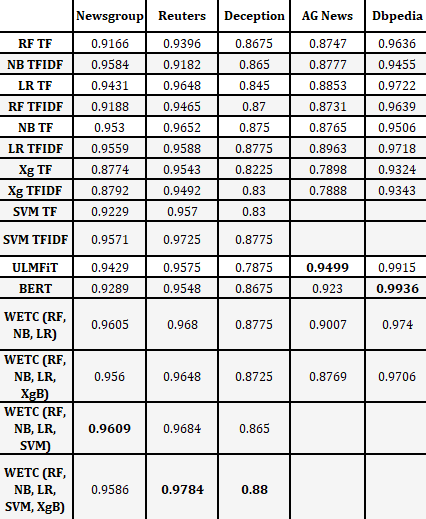
\includegraphics[width=0.75\textwidth]{images/wetc.png}
    \caption{Weighted Ensemble of Text Classifiers Result}
    \label{fig:wetc_res}
\end{figure}


% The results from \cref{tab:azoth_res1} suggest that the hand crafted deep learning methods are equally better as of the linguistic features. The graph from the \cref{fig:azoth_res1} and \cref{fig:azoth_res2} suggest that with the increase in data, the performance of the model changes as well. We can see the class imbalance problem from the \cref{fig:azoth_res1} and \cref{fig:azoth_res2} when in the last step, where whole data is being used for training we can see a drop in macro f1 score where as a rise in the accuracy. This is due to the fact that the dataset is heavily imbalanced (1500 examples for accept, 600 for postpone and 400 for reject).

% \begin{figure}
%     \centering
%     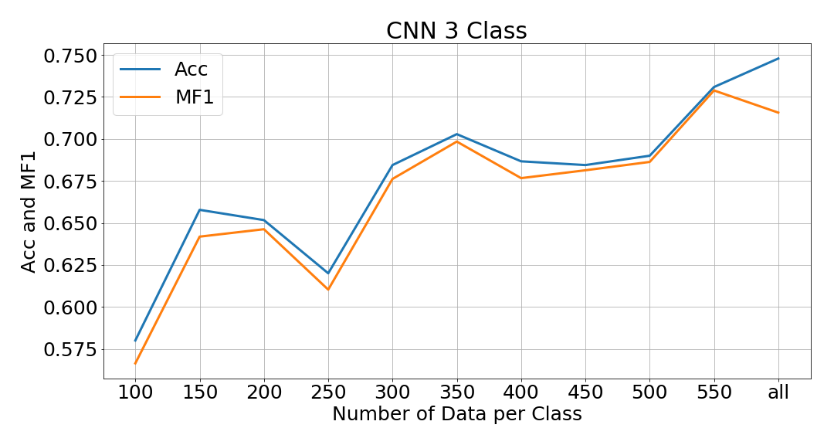
\includegraphics[width=\textwidth]{images/cnn3class.png}
%     \caption{CNN change in performance w.r.t change in data per class in 3 class problem}
%     \label{fig:azoth_res1}
% \end{figure}

% \begin{figure}
%     \centering
%     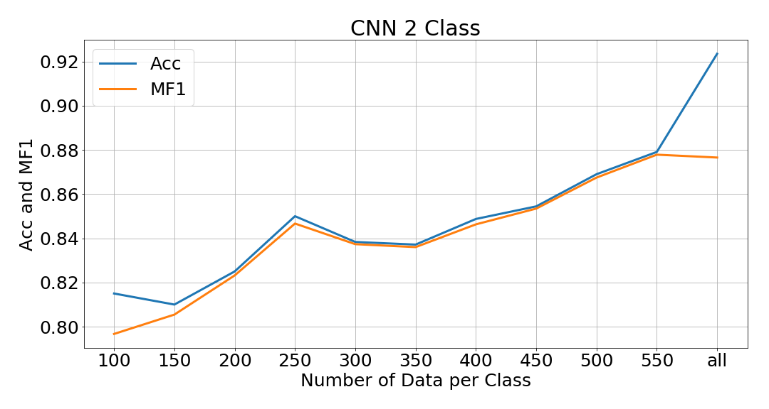
\includegraphics[width=\textwidth]{images/cnn2.png}
%     \caption{CNN change in performance w.r.t change in data per class in accept vs reject}
%     \label{fig:azoth_res2}
% \end{figure}


% \clearpage

\section{Identified Impact}\label{sec:impact}
This research will introduce new state-of-the-art methodologies for solving the NLP related problems in business processes. Machine learning research has evolved rapidly with the introduction of deep learning techniques build upon the support of tremendous computational power. But still there use in business processes is very few due to the difference between nature of problems in real-world applications and academic research. We will bring attention to the academic research community towards the problems faced by business processes that are not well addressed right now. Our work will help industries make their workforce allocation better as many tasks which do not need much human intervention will be handled in an automated manner. This will free up the human resource of a company for more creative and innovate tasks. Eventually leading in the cost reduction as they have to focus on quality of their workforce instead of quantity.

Right now the work done by few industries to automate their business process is not made available in public domain. There are a few conglomerates who work on developing methods to address some of their problems but they tend not to open-source their findings in order to gain financial profits. The findings from our project will be made public through various publications and code sharing website like GitHub \footnote{\url{https://github.com/}} that can help industries with lesser resources to enhance their performance. Instead of using their resources on automating their text related processes they can focus on their core issues \& ideas whereas our work can help them in automation.

% We plan to build upon current
% deep learning techniques on HAR, adapt and improve them for multi-modal sensor reasoning for exercises.
% With objective 1 we will bring together different machine learning data domains such as time
% series, images and video as we create a multi-modal spatio-temporal dataset. It will be adaptable to
% different application domains as well as future research in HAI. It will also contribute towards evaluating
% transfer learning capabilities of machine learning models. Objective 2 will introduce new attention
% mechanisms for sensor data selection in abstract levels and in objective 3 we will introduce strategies
% to improve robustness in deep learning architectures.Objective 4 will implement novel deep learning
% models for qualitative evaluation which involves similarity comparison of spatio-temporal data.
% From the healthcare application perspective this research will contribute towards a sustainable
% digital intervention for MSD prevention and self-management while raising awareness. MSD has
% directly affects the workforce of a country with sedentary lifestyles and as a result it has a major
% impact on economical and social status of the country. This digital intervention will enable the user
% to perform physiotherapist recommended exercises at home with supervision from the qualitative
% evaluation component. We plan to involve users in each step of this research and raise awareness. We
% will seek user feedback on the utility of the digital intervention to support, maintain and encourage
% an active lifestyle in the prevention and management of MSDs

% The major outcome expected of this project is the development and production
% of a sustainable profile generation and long term health condition risk determination system, designed to scale with additional FitHomes installations as they
% are constructed. As new residents move into homes, labelled examples will be
% produced with a slight involvement on their end, ensuring personalised profiles
% are produced based on their regular performances of activities. Bespoke and
% retrofit sensor environments will also be supported. This will ensure that the
% FitHomes project can safely expand and continue to provide state-of-the-art
% sensor analytics to residents.
% It was proposed that 2-3 impactful publications may be produced as a result
% of this project. In the long term, we can expect the FitHomes project as a whole
% will provide a very useful unique dataset for data mining. This may potentially
% allow for future research on seemingly unrelated and unknown risk factors for a
% range of long term health conditions to be highlighted. Other long term studies
% in home environments may also be able to make use of any publicly distributed
% FitHomes datasets which would have a high impact in the field. Multi-modal
% sensor analytics as a field could benefit from this project.


% This will help several industries to automate their process in various domains

% \clearpage

\section{Time Management Plan}\label{sec:time_plan}
% ``In Progress''

\newcounter{loopcntr}
\newcommand{\onblue}[1][1]{
  \forloop{loopcntr}{0}{\value{loopcntr}<#1}{&\cellcolor{blue}}
}
\newcommand{\onbluee}[1][1]{
  \forloop{loopcntr}{0}{\value{loopcntr}<#1}{&\cellcolor{bluee}}
}
\newcommand{\off}[1][1]{
  \forloop{loopcntr}{0}{\value{loopcntr}<#1}{&}
}
\definecolor{blue}{HTML}{002b80}
\definecolor{bluee}{HTML}{ccddff}

\noindent\begin{tabular}
{|p{0.54\textwidth}
!{\vrule width 0.4mm}p{0.01\textwidth}*{3}{|p{0.01\textwidth}}
!{\vrule width 0.4mm}p{0.01\textwidth}*{3}{|p{0.01\textwidth}}
!{\vrule width 0.4mm}p{0.01\textwidth}*{3}{|p{0.01\textwidth}}
|}

\hline
\textbf{Time Management Plan} 
& \multicolumn{4}{c!{\vrule width 0.4mm}}{Year 1} 
& \multicolumn{4}{c!{\vrule width 0.4mm}}{Year 2} 
& \multicolumn{4}{c!{\vrule width 0.4mm}}{Year 3} \\

\hline
\textbf{Objective 1} & \multicolumn{12}{c|}{} \\
\hline
Review literature to identify the research gaps \onblue[3] \onbluee[7] \off[2] \\
% \hline
% Contemplation for identifying the research gaps \off[1] \onblue[2] \onbluee[3] \off[6] \\
\hline
Talking to industry representatives for identifying gaps \off[2] \onblue[2] \onbluee[3] \off[5] \\
\hline
\textbf{Objective 2} & \multicolumn{12}{c|}{} \\
\hline
Identifying use-case and gathering data  \off[3] \onblue[2] \onbluee[3] \off[4] \\
\hline
\textbf{Objective 3} & \multicolumn{12}{c|}{} \\
\hline
Implementing state-of-the-arts methods on gathered data \off[4] \onblue[4] \onbluee[2] \off[2] \\
\hline
\textbf{Objective 4} & \multicolumn{12}{c|}{} \\
\hline
Proposing new algorithms to outperform the benchmark performance \off[6] \onblue[4] \onbluee[2] \\
\hline
Evaluating proposed methods on real-world data \off[7] \onblue[4] \onbluee[1] \\
\hline
\textbf{Final} & \multicolumn{12}{c|}{} \\
\hline
Finalizing Thesis Submission \off[10] \onblue[2] \\
\hline

\end{tabular}

\clearpage


\bibliographystyle{agsm}
\bibliography{ref}
\clearpage

\begin{appendices}

% \section{Sensor Fusion with SelfBACK}
% \label{appendix:selfback}
% \input{misc/selfback_results}

\section{Vitae Personal Development Planner}
\label{appendix:vitae}
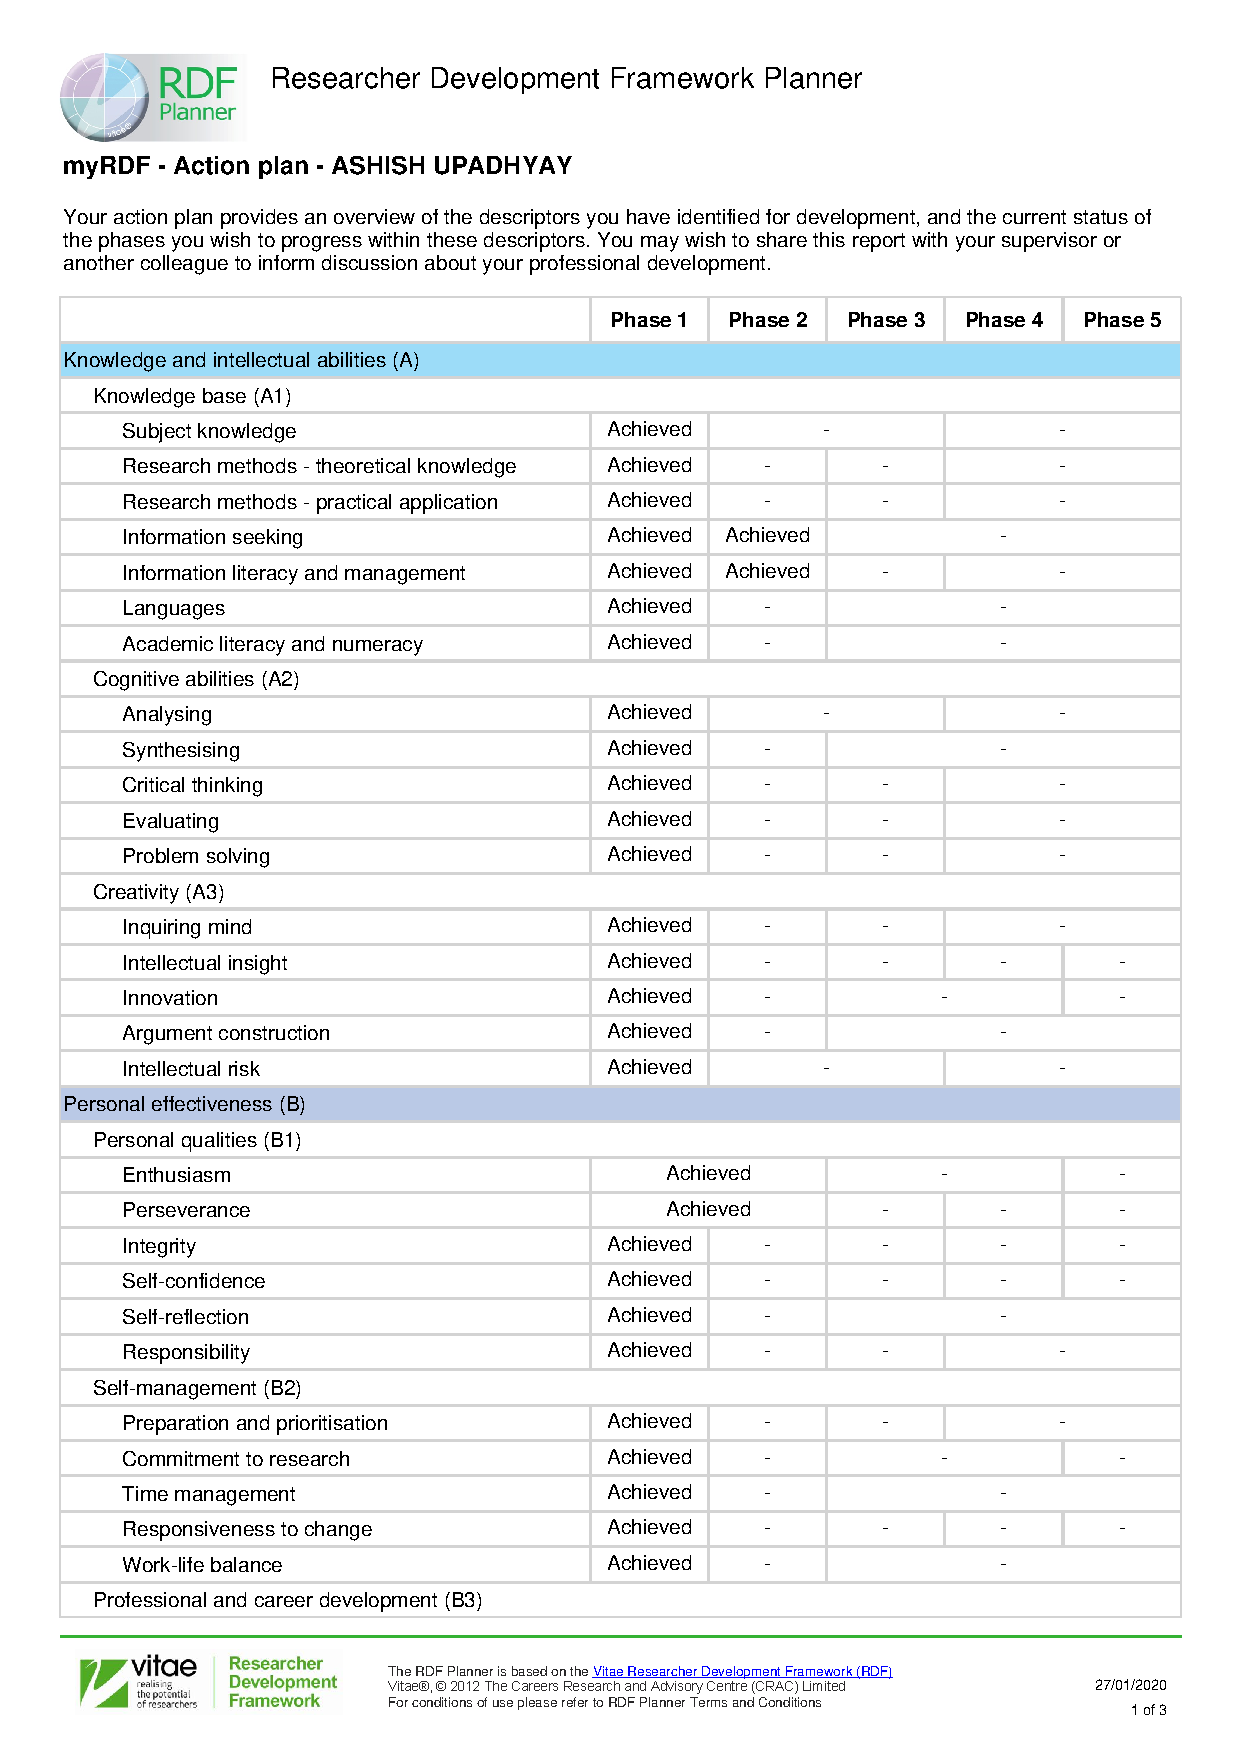
\includepdf[pages={1-3}]{misc/action_plan.pdf}

\end{appendices}

\end{document}
